\documentclass[11pt]{article}

%% ---------------------------------------------------------------
%% Page layout and fonts
%% ---------------------------------------------------------------
\usepackage[a4paper,top=2.5cm,bottom=2.5cm,left=2.5cm,right=2.5cm,headheight=14pt]{geometry}
\usepackage{fontspec}
\setmainfont{LibertinusSerif}[Extension=.otf,UprightFont=*-Regular,BoldFont=*-Bold,ItalicFont=*-Italic,BoldItalicFont=*-BoldItalic]
\usepackage{unicode-math}
\setmathfont{LibertinusMath-Regular.otf}
\usepackage{microtype}
\usepackage{setspace}
\onehalfspacing
\setlength{\parindent}{1.5em}
\setlength{\parskip}{0pt}
\emergencystretch=3em
\clubpenalty=10000
\widowpenalty=10000

%% ---------------------------------------------------------------
%% Packages
%% ---------------------------------------------------------------
\usepackage{amsmath}
\usepackage{graphicx}
\usepackage{booktabs,longtable,array,calc}
\usepackage[table]{xcolor}
\usepackage[most]{tcolorbox}
\usepackage{enumitem}
\usepackage{float}
\usepackage[mathlines]{lineno}
\usepackage{fancyhdr}
\usepackage{titlesec}
\usepackage{caption}
\usepackage{xurl}
\usepackage[hidelinks]{hyperref}
\urlstyle{same}
\hypersetup{
  pdftitle={The evaluation gap in single-cell cancer genomics: a quantitative review, benchmark catalogue and ground-truth resource},
  pdfauthor={Md. Jubayer Hossain},
  pdfkeywords={single-cell RNA sequencing; cancer genomics; benchmarking; meta-research; ground truth; calibration; multiverse analysis}
}

%% ---------------------------------------------------------------
%% Headings (sections are numbered manually in the text)
%% ---------------------------------------------------------------
\setcounter{secnumdepth}{0}
\titleformat{\section}{\normalfont\large\bfseries}{}{0pt}{}
\titleformat{\subsection}{\normalfont\normalsize\bfseries}{}{0pt}{}
\titleformat{\subsubsection}{\normalfont\normalsize\itshape}{}{0pt}{}
\titlespacing*{\section}{0pt}{1.6ex plus .4ex minus .2ex}{0.8ex plus .2ex}
\titlespacing*{\subsection}{0pt}{1.2ex plus .3ex minus .2ex}{0.5ex plus .1ex}
\titlespacing*{\subsubsection}{0pt}{1.0ex plus .3ex minus .2ex}{0.3ex plus .1ex}

%% ---------------------------------------------------------------
%% Header / footer
%% ---------------------------------------------------------------
\pagestyle{fancy}
\fancyhf{}
\fancyhead[R]{\small\itshape The evaluation gap in single-cell cancer genomics}
\fancyfoot[C]{\small\thepage}
\renewcommand{\headrulewidth}{0pt}
\fancypagestyle{plain}{\fancyhf{}\fancyfoot[C]{\small\thepage}\renewcommand{\headrulewidth}{0pt}}

%% ---------------------------------------------------------------
%% Floats, captions and tables
%% ---------------------------------------------------------------
\captionsetup{font={small,stretch=1.1},labelformat=empty,justification=justified,singlelinecheck=false,skip=6pt}
\captionsetup[longtable]{font={small,stretch=1.1},labelformat=empty,justification=justified,singlelinecheck=false,skip=4pt}
\floatplacement{figure}{!htbp}
\makeatletter\def\fps@figure{!htbp}\makeatother
\renewcommand{\topfraction}{0.9}
\renewcommand{\bottomfraction}{0.8}
\renewcommand{\textfraction}{0.07}
\renewcommand{\floatpagefraction}{0.75}
\setkeys{Gin}{width=\linewidth,height=0.62\textheight,keepaspectratio}
\setlength{\LTcapwidth}{\textwidth}
\setlength{\LTpre}{6pt}
\setlength{\LTpost}{6pt}
\renewcommand{\arraystretch}{1.2}
\newenvironment{tablefont}{\par\scriptsize\setlength{\tabcolsep}{3.5pt}\nolinenumbers}{\par\linenumbers}
\newcommand{\thead}[1]{\textbf{#1}}

%% ---------------------------------------------------------------
%% Lists and pandoc compatibility
%% ---------------------------------------------------------------
\setlist{noitemsep,topsep=3pt,leftmargin=*}
\providecommand{\tightlist}{\setlength{\itemsep}{0pt}\setlength{\parskip}{0pt}}
\providecommand{\pandocbounded}[1]{#1}

\begin{document}

%% ===============================================================
%% Title page
%% ===============================================================
\begin{titlepage}
\thispagestyle{empty}
\begin{flushleft}
\setstretch{1.15}
{\Large\bfseries\hyphenpenalty=10000
The evaluation gap in single-cell cancer genomics: a quantitative review, benchmark catalogue and ground-truth resource\par}
\vspace{2em}
{\large Md.\ Jubayer Hossain\textsuperscript{1,2,*}\par}
\vspace{1.2em}
{\small
\textsuperscript{1}Center for Health Innovation, Research, Action, and Learning -- Bangladesh (CHIRAL Bangladesh), Dhaka, Bangladesh\par
\textsuperscript{2}DeepBio, Dhaka, Bangladesh\par}
\vspace{1.5em}
{\small
\textsuperscript{*}\textbf{Correspondence:} Md.\ Jubayer Hossain\\
E-mail: \href{mailto:contact.jubayerhossain@gmail.com}{contact.jubayerhossain@gmail.com}\par}
\vspace{2.5em}
\renewcommand{\arraystretch}{1.3}
{\small
\begin{tabular}{@{}p{0.27\textwidth}p{0.69\textwidth}@{}}
\textbf{Running title} & The evaluation gap in single-cell cancer genomics\\
\textbf{Article type} & Review (quantitative review and resource)\\
\textbf{Abstract} & 303 words\\
\textbf{Main text} & 6,280 words (Introduction to Conclusions, excluding tables, legends and references)\\
\textbf{Display items} & 6 figures, 6 tables, 1 box\\
\textbf{References} & 121\\
\textbf{Supplementary data} & S1--S9\\
\end{tabular}}
\end{flushleft}
\end{titlepage}

\linenumbers

\section{Abstract}\label{abstract}
\begingroup\setlength{\parindent}{0pt}\setlength{\parskip}{0.6ex}

\textbf{Background.} Single-cell cancer genomics grew from 443 PubMed
records in 2015 to 7,556 in 2025. Whether evaluation of its
computational methods has kept pace has not been quantified.

\textbf{Methods.} We combined a 26-topic PubMed volume series (2015 to
15 October 2026); verification of all 486 evaluation-titled papers with
an independent second coding pass; a catalogue of 269 PubMed-verified
benchmarks in 16 method classes, coded for ground-truth strategy and for
assessment of robustness, calibration and metric validity; a
catalogue of 1,336 GEO tumour single-cell series carrying orthogonal
validation data; and explicit-definition coding of a stratified sample of 1,771 unique abstracts (150 draws per year, 2015--2026). Rates were modelled by
negative-binomial and Poisson regression.

\textbf{Results.} Of 486 evaluation-titled papers, 158 (32.5\%; 95\% CI
28.5--36.8) were genuine benchmarks (inter-pass κ = 0.74). Benchmarks
per 1,000 papers declined by 7.8\% per year (rate ratio 0.922,
0.875--0.972); the decline was concentrated in biology and application
topics (0.90 per year, 0.84--0.97), whereas method topics were flat.
Over 2015--2026, method topics received more benchmarks per paper (IRR
2.35, 1.66--3.31). ``No ground truth'', the most frequently coded
limitation (24.2\%), did not replicate on re-coding (κ ≈ 0) and was
stated in 1.1\% of abstracts under an explicit definition. Abstracts
stating any evaluation-check problem fell from 14.0\% (2015--18) to
3.6\% (2024--26). Robustness to analytical choices was reported in 5.6\%
of benchmarks, calibration in 3.3\% and metric validity in 3.0\%; metric
validity was reported in none of the 48 cancer-specific benchmarks.
Public validation data are more widely available than used: 138 series
carry matched exomes, 227 CITE-seq protein and 250 paired spatial data,
whereas 44 benchmarks state an orthogonal-assay ground truth.

\textbf{Conclusions.} Evaluation in this field is limited less by absent
ground truth than by rarely performed checks and under-used public
validation data. We release both catalogues, a ten-item evaluation
standard and an eight-study research agenda.

\textbf{Keywords:} single-cell RNA sequencing; cancer genomics;
benchmarking; meta-research; ground truth; calibration; multiverse
analysis

\endgroup
\clearpage
\section{1. Introduction}\label{introduction}

Biological conclusions drawn from tumour single-cell data depend on a
sequence of computational decisions. The identification of malignant
cells, the integration of patients, the reference used to label the
immune compartment and the inference of cell-type proportions or
interactions are each delegated to software. That software typically
returns point estimates; in the benchmark literature catalogued here,
calibration or uncertainty is assessed in 3.3\% of studies (§3.4).
Principles for evaluating such software are nevertheless established.
Neutral comparison studies {[}1{]} should be designed to avoid the
self-assessment trap, in which developers rank their own method best
{[}2,3{]}. They should follow explicit design guidelines {[}4,5{]} and
be extensible as methods change {[}6,7{]}. Landmark neutral benchmarks
exist for many single-cell tasks, including clustering {[}8{]},
differential expression {[}9,10{]}, trajectory inference {[}11{]},
annotation {[}12{]}, batch correction {[}13,14{]}, doublet detection
{[}15{]}, cell--cell communication {[}16{]}, spatial integration
{[}17{]}, deconvolution {[}18{]} and perturbation prediction {[}19{]}.

Two questions remain open. The first is whether this evaluation effort
has reached cancer-specific applications; tumour microenvironment
composition alone accounted for 9,383 papers in 2023--26 (Table 1). The
second is whether it addresses the failure modes specific to tumour
data. Malignant cells show extensive inter- and intratumoural
transcriptional heterogeneity, with 41 recurrent meta-programmes
identified across 1,163 tumour samples {[}20--22{]}. Copy-number
alterations, which are absent from normal tissue, are themselves
inferred from expression {[}20,23,24{]}. Reference atlases used for
annotation are built predominantly from non-malignant tissue {[}25{]}.
None of these properties is represented in benchmarks that use only
non-malignant data. Yet only 48 of the 269 benchmarks catalogued here
(17.8\%) are cancer-specific (§3.4).

This review quantifies the evaluation gap. We quantify how benchmark
coverage has scaled with publication volume across 26 subtopics and test
whether coverage is shrinking. We then ask what the literature says is
wrong, and check whether those statements survive independent coding.
Next we catalogue what existing benchmarks actually check, and locate
where ground truth already exists in public repositories. Section 4
synthesises the state of evaluation for each major method class. Section
5 develops the three checks that the evidence identifies as most
neglected: metric validity, robustness to analytical choices, and
calibration. Section 6 maps the public ground-truth resource. Sections 7
and 8 propose a minimum evaluation standard and a research agenda. The
benchmark catalogue, ground-truth catalogue and all derived tables are
released with the paper.

\section{2. Methods}\label{methods}

\subsection{2.1 Taxonomy, volume series and corpus}\label{taxonomy-volume-series-and-corpus}

We defined 26 subtopics of single-cell cancer genomics spanning methods
and measurement (for example CNV inference and scDNA-seq, integration,
lineage tracing, spatial transcriptomics) and biology and application
(for example immunotherapy response, tumour microenvironment
composition, metastasis). For each topic and for the subfield as a
whole, we retrieved annual PubMed record counts for 2015--2026 through
NCBI E-utilities, giving 324 topic-year counts. Counts for 2026 run to
15 October 2026 (§2.7). We summarise growth as the ratio of a topic's
2025 share of the subfield to its 2021 share. Abstracts for 2023--2026
(n = 3,627) were harvested with topic tags; topics overlap and are not a
partition. A bioRxiv screen (15,682 preprints, 18 months) yielded 372
single-cell cancer preprints. Because the bioRxiv API exposes only a
short abstract preview, preprint ratios are not used inferentially here.

\subsection{2.2 Benchmark verification and problem extraction}\label{benchmark-verification-and-problem-extraction}

All 486 papers whose titles contained ``benchmark'', ``comparison'',
``evaluation'' or ``assessment'' were classified from their abstracts as
genuine methods benchmarks or not. A genuine benchmark is a systematic
comparison of two or more named tools or platforms on a shared task.
Separately, each abstract in the corpus was coded for its stated
limitations and open problems into a 17-category controlled vocabulary,
giving 1,757 extraction rows. Of these, 1,506 were methodological
problems.

\subsection{2.3 Reliability of the coding}\label{reliability-of-the-coding}

Both coding tasks were repeated blind to the first-pass labels, using a
reworded prompt and a different model tier. A smaller model (Haiku-tier)
rated 394 of the 486 benchmark abstracts. After that model's token
budget was exhausted, the remaining 92 benchmark abstracts and the
entire random subsample of 200 problem-coded abstracts (seed 1) were
rated from condensed abstracts (title, opening and closing sentences) by
the coordinating language-model agent that ran the analysis. That agent
did not see the first-pass labels, but it is not an independent human
coder, and no human adjudication was performed. We report Cohen's κ with
bootstrap 95\% intervals separately by rater subset. Second-pass counts
are from one non-adjudicated pass and are treated as provisional.

\subsection{2.4 Stated problems, 2015--2026}\label{stated-problems-20152026}

The archived abstract corpus covers 2023--2026 and is weighted towards
recent records (2,073 of its 3,627 abstracts were first published in
2026, as confirmed by re-dating every record against PubMed). To examine
change over time, we drew a stratified random sample of 150 research
abstracts per publication year from 2015 to 2026 (seed 2026) from the
subfield query, excluding reviews, editorials, comments and errata and
requiring an abstract of at least 400 characters. Each abstract was
coded by a model coder (Haiku-class, temperature 0, structured output,
15 abstracts per request) with written definitions for 17 problem types
(Table 3); a problem type was coded only when the abstract explicitly
stated it, and multiple types per abstract were allowed. The coder also
flagged whether the study generated or analysed single-cell omics data,
as distinct from flow cytometry, imaging or other non-sequencing
single-cell assays. Because PubMed's publication-date field matches both
electronic and print years, 29 papers were drawn in two adjacent years;
each was counted once, in its earlier year, leaving 1,771 unique
abstracts. Analyses were restricted to abstracts flagged as single-cell
omics. A random 150 of the coded abstracts were re-coded independently
by a stronger model (Sonnet-class) with the same definitions to estimate
agreement. The 158 verified benchmarks were flagged for single-cell
omics in the same way.

\subsection{2.5 Benchmark catalogue}\label{benchmark-catalogue}

We assembled a catalogue of benchmark studies relevant to single-cell
cancer genomics. Sources were the verified first-pass benchmarks within
scope, 16 class-specific PubMed queries, about 90 targeted searches for
landmark benchmarks, and 14 supplementary queries. Inclusion required
that the primary contribution be a comparative evaluation of at least
two existing methods, or of platforms with computational read-outs;
preprint and journal versions were merged. All 269 records were resolved
through PubMed efetch and re-checked by esummary title match. Evaluation
fields were coded from abstracts by keyword rules, with manual
correction of 40 records including all landmark records. The fields are
the ground-truth strategy, the number of tools, and whether robustness
to parameters, calibration or uncertainty, and the validity of the
metric itself were assessed. A field is marked as assessed only when the
abstract says so. All assessment counts are therefore lower bounds.

\subsection{2.6 Ground-truth catalogue}\label{ground-truth-catalogue}

We queried GEO DataSets for human tumour single-cell series. The base
set held 6,141 series, and the union of nine modality queries gave 2,715
records. After filtering to sequencing-based, human, single-cell, cancer
series, 2,024 were eligible. From series-level text we classified nine
validation modalities: matched WES/WGS, CITE-seq protein, genotype or
hashtag multiplexing, paired bulk RNA, paired spatial, mtDNA lineage,
longitudinal or on-treatment sampling, cell-line mixtures and
Perturb-seq. Classification used documented, spot-audited
regular-expression rules. The result is 1,336 validation-bearing series
in 1,166 SuperSeries-collapsed study groups. Each series was mapped to
the benchmark tasks it can support. A modality call means the submitters
state that the data were generated. Controlled-access deposition
(dbGaP/EGA) was not checked, recall was not measured, and ArrayExpress,
HTAN and CELLxGENE were not searched.

\subsection{2.7 Update of 2026 counts to 15 October 2026}\label{update-of-2026-counts-to-15-october-2026}

The volume series was first retrieved on 4 October 2026. To extend 2026
to 15 October 2026 without altering the 2015--2025 series, we
reconstructed the subfield query and calibrated it against the archived
counts: it reproduced every year from 2015 to 2025 within ±0.7\% (for
example, 442 versus 443 records in 2015 and 7,528 versus 7,556 in 2025).
For each topic we selected, from two or three candidate clauses, the one
that best reproduced the archived 2017, 2021 and 2025 counts. For every
series we then counted 2026 records with an Entrez date up to 4 October
and all 2026 records on 15 October using the same reconstructed query,
and multiplied the archived 2026 count by this growth ratio, so that
differences between the reconstructed and original queries cancel.
Growth ratios ranged from 1.014 to 1.064 across topics and were 1.031
for the subfield, which rose from 7,342 to 7,571 records. The same title
query identified three evaluation-titled 2026 records indexed after 4
October; none was a methods benchmark, so the verified 2026 benchmark
count remains 25. All models in §2.8 were refitted on the updated
denominators. Queries, counts and ratios are released in Supplementary
Data S7.

\subsection{2.8 Statistical analysis}\label{statistical-analysis}

Proportions carry Wilson score 95\% intervals; benchmark rates per 1,000
papers carry exact Poisson intervals. Per-topic benchmark counts were
modelled with NB2 negative-binomial regression, with an offset of log
topic volume (2015--26 in the primary specification) and two covariates.
One is log share change (2025 vs 2021). The other is an indicator for
method and measurement topics, whose mapping and rationale are released
with the paper. Sensitivity fits excluded the benchmarking topic itself,
restricted numerator and offset to 2023--26, and used an alternative
topic coding. Poisson fits are reported where the LR test for
overdispersion was not significant. The temporal trend was modelled as a
Poisson GLM of verified benchmarks per year with an offset of log
subfield volume (2015--2026), with binomial and NB2 sensitivity fits and
a 2015--2025 fit that excludes the partial year. Topic-level coverage
was analysed over the full window (benchmarks and papers 2015 to 15
October 2026) as the primary specification, with the 2023--26 window as
a sensitivity analysis. To locate the temporal decline, we fitted a
Poisson model to topic-by-year benchmark counts with topic fixed
effects, an offset of log topic-year volume and separate year slopes for
method and biology topics, excluding the benchmarking topic. As
sensitivity analyses for the subfield trend and the panel, numerators
were restricted to single-cell-genomics benchmarks and denominators were
multiplied by the yearly single-cell-omics share estimated from the
stratified sample (§2.4). Prevalence trends in stated problems were
tested by logistic regression on publication year. Before writing, 120
quantities quoted in our earlier gap analysis were recomputed from the
archived data. 101 matched exactly and one matched approximately. Six
did not match: preprint-ratio denominators, one rounded range, and a
numerator-window inconsistency discussed in §3.2. Twelve could not be
checked from archived data, and none of those twelve is used here.

\subsection{2.9 Reference verification}\label{reference-verification}

Every work cited was resolved to its PubMed or Crossref record (one
machine-learning conference paper via arXiv). For foundational
references, the claim attributed to each work was checked against its
abstract and rewritten where it was not supported as first stated.
Records that could not be resolved were dropped rather than cited from
memory.

\section{3. Results}\label{results}

\subsection{3.1 A fast-growing field whose growth is in applications}\label{a-fast-growing-field-whose-growth-is-in-applications}

The subfield grew 17-fold between 2015 and 2025 (Fig. 1a; Table 1) and
had already reached 7,571 records by 15 October 2026, a full-year pace
of about 9,600. All 26 topics grew in absolute terms, but share moved
sharply. Spatial transcriptomics in tumours gained share 6.2-fold
between 2021 and 2025. Drug-response prediction gained 3.2-fold, deep
learning and foundation models 3.1-fold, and cell--cell communication
2.3-fold. The topics losing share were mature method areas: clonal
evolution and phylogeny (0.44×), CTC and liquid biopsy (0.46×),
intratumour-heterogeneity metrics (0.67×) and lineage tracing (0.68×)
(Fig. 1c). Benchmarking and evaluation as a topic accounted for 87
papers in 2025.

\begin{figure}[!htbp]
\centering
\pandocbounded{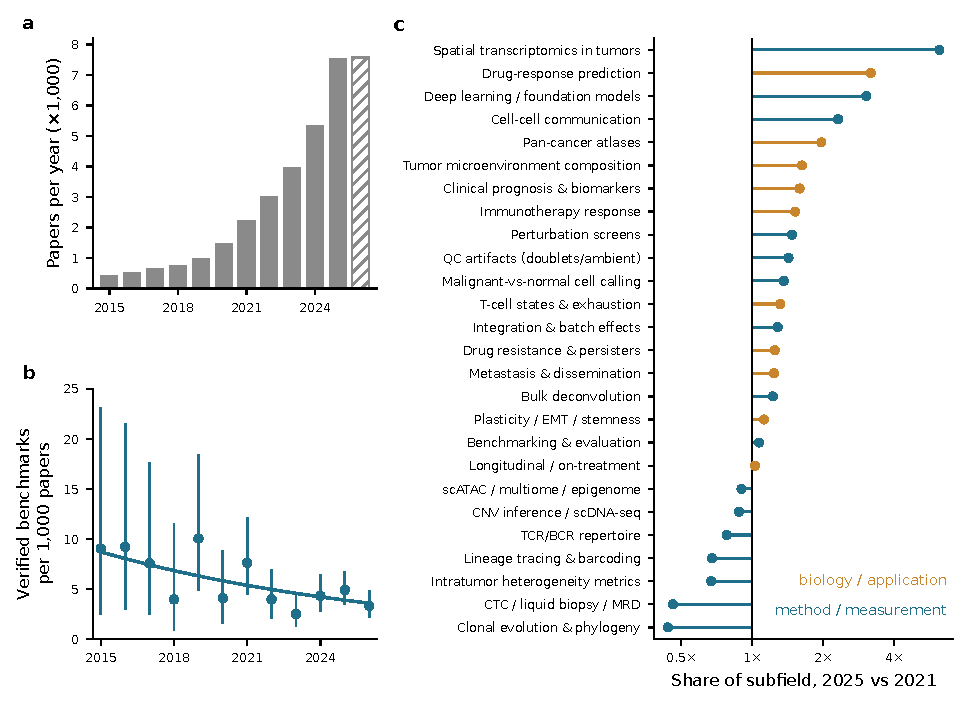
\includegraphics[keepaspectratio,alt={Figure 1. Growth of
single-cell cancer genomics and decline in benchmark coverage. (a)
Annual PubMed records for the subfield, 2015--2026; the subfield grew
17-fold between 2015 (443) and 2025 (7,556). The hatched 2026 bar covers
1 January--15 October (7,571 records). (b) Verified methods benchmarks
per 1,000 subfield papers by publication year, with exact Poisson 95\%
intervals (n = 12 years, 157 benchmarks). The line is the fitted Poisson
trend with an offset of log subfield volume: rate ratio 0.922 per year
(95\% CI 0.875--0.972; p = 0.0027). (c) Ratio of each topic's 2025 share
of the subfield to its 2021 share (log scale; 1× marks growth equal to
the subfield). Colour indicates the method/measurement versus
biology/application classification used in the coverage model. Spatial
transcriptomics gained the most share (6.2×) and clonal evolution and
phylogeny lost the most (0.44×).}]{fig/fig1_landscape.pdf}}
\caption{\textbf{Figure 1. Growth of single-cell cancer genomics and
decline in benchmark coverage.} (a) Annual PubMed records for the
subfield, 2015--2026; the subfield grew 17-fold between 2015 (443) and
2025 (7,556). The hatched 2026 bar covers 1 January--15 October (7,571
records). (b) Verified methods benchmarks per 1,000 subfield papers by
publication year, with exact Poisson 95\% intervals (n = 12 years, 157 benchmarks). The line is the fitted Poisson trend with an offset of log
subfield volume: rate ratio 0.922 per year (95\% CI 0.875--0.972; p =
0.0027). (c) Ratio of each topic's 2025 share of the subfield to its
2021 share (log scale; 1× marks growth equal to the subfield). Colour
indicates the method/measurement versus biology/application
classification used in the coverage model. Spatial transcriptomics
gained the most share (6.2×) and clonal evolution and phylogeny lost the
most (0.44×).}
\end{figure}

\begin{tablefont}

\begin{longtable}[l]{@{}
  >{\raggedright\arraybackslash}p{(\linewidth - 14\tabcolsep) * \real{0.2857}}
  >{\raggedright\arraybackslash}p{(\linewidth - 14\tabcolsep) * \real{0.1786}}
  >{\raggedright\arraybackslash}p{(\linewidth - 14\tabcolsep) * \real{0.0714}}
  >{\raggedright\arraybackslash}p{(\linewidth - 14\tabcolsep) * \real{0.0714}}
  >{\raggedright\arraybackslash}p{(\linewidth - 14\tabcolsep) * \real{0.1071}}
  >{\raggedright\arraybackslash}p{(\linewidth - 14\tabcolsep) * \real{0.0714}}
  >{\raggedright\arraybackslash}p{(\linewidth - 14\tabcolsep) * \real{0.1071}}
  >{\raggedright\arraybackslash}p{(\linewidth - 14\tabcolsep) * \real{0.1071}}@{}}
\caption{\textbf{Table 1.} Topic taxonomy and growth. PubMed records per topic;
topics overlap. Share change is the ratio of the 2025 to the 2021 share
of the subfield. 2026 counts run to 15 October 2026.}\tabularnewline
\toprule
\begin{minipage}[b]{\linewidth}\raggedright
\thead{Topic}
\end{minipage} & \begin{minipage}[b]{\linewidth}\raggedright
\thead{Class}
\end{minipage} & \begin{minipage}[b]{\linewidth}\raggedright
\thead{2021}
\end{minipage} & \begin{minipage}[b]{\linewidth}\raggedright
\thead{2025}
\end{minipage} & \begin{minipage}[b]{\linewidth}\raggedright
\thead{2026 (to 15 Oct)}
\end{minipage} & \begin{minipage}[b]{\linewidth}\raggedright
\thead{2023--26}
\end{minipage} & \begin{minipage}[b]{\linewidth}\raggedright
\thead{CAGR 2021--25}
\end{minipage} & \begin{minipage}[b]{\linewidth}\raggedright
\thead{Share change}
\end{minipage} \\
\midrule
\endfirsthead
\toprule
\begin{minipage}[b]{\linewidth}\raggedright
\thead{Topic}
\end{minipage} & \begin{minipage}[b]{\linewidth}\raggedright
\thead{Class}
\end{minipage} & \begin{minipage}[b]{\linewidth}\raggedright
\thead{2021}
\end{minipage} & \begin{minipage}[b]{\linewidth}\raggedright
\thead{2025}
\end{minipage} & \begin{minipage}[b]{\linewidth}\raggedright
\thead{2026 (to 15 Oct)}
\end{minipage} & \begin{minipage}[b]{\linewidth}\raggedright
\thead{2023--26}
\end{minipage} & \begin{minipage}[b]{\linewidth}\raggedright
\thead{CAGR 2021--25}
\end{minipage} & \begin{minipage}[b]{\linewidth}\raggedright
\thead{Share change}
\end{minipage} \\
\midrule
\endhead
\bottomrule
\endlastfoot
Spatial transcriptomics in tumors & method/measurement & 46 & 970 &
1,413 & 3,030 & 114\% & 6.23× \\
Drug-response prediction & biology/application & 128 & 1,382 & 1,429 &
3,920 & 81\% & 3.19× \\
Deep learning / foundation models & method/measurement & 100 & 1,033 &
1,125 & 2,996 & 79\% & 3.05× \\
Cell-cell communication & method/measurement & 84 & 659 & 865 & 2,196 &
67\% & 2.32× \\
Pan-cancer atlases & biology/application & 68 & 453 & 404 & 1,393 & 61\%
& 1.97× \\
Tumor microenvironment composition & biology/application & 528 & 2,908 &
3,189 & 9,383 & 53\% & 1.63× \\
Clinical prognosis \& biomarkers & biology/application & 803 & 4,327 &
4,282 & 13,532 & 52\% & 1.59× \\
Immunotherapy response & biology/application & 450 & 2,322 & 2,356 &
7,558 & 51\% & 1.53× \\
Perturbation screens & method/measurement & 7 & 35 & 40 & 109 & 50\% &
1.48× \\
QC artifacts (doublets/ambient) & method/measurement & 18 & 87 & 115 &
275 & 48\% & 1.43× \\
Malignant-vs-normal cell calling & method/measurement & 76 & 351 & 445 &
1,213 & 47\% & 1.37× \\
T-cell states \& exhaustion & biology/application & 276 & 1,228 & 1,413
& 4,103 & 45\% & 1.32× \\
Integration \& batch effects & method/measurement & 23 & 100 & 136 & 324
& 44\% & 1.29× \\
Drug resistance \& persisters & biology/application & 161 & 680 & 663 &
1,964 & 43\% & 1.25× \\
Metastasis \& dissemination & biology/application & 439 & 1,842 & 1,884
& 5,716 & 43\% & 1.24× \\
Bulk deconvolution & method/measurement & 62 & 257 & 332 & 846 & 43\% &
1.23× \\
Plasticity / EMT / stemness & biology/application & 202 & 768 & 1,027 &
2,636 & 40\% & 1.12× \\
Benchmarking \& evaluation & method/measurement & 24 & 87 & 108 & 283 &
38\% & 1.07× \\
Longitudinal / on-treatment & biology/application & 54 & 188 & 295 & 681
& 37\% & 1.03× \\
scATAC / multiome / epigenome & method/measurement & 56 & 171 & 201 &
573 & 32\% & 0.90× \\
CNV inference / scDNA-seq & method/measurement & 107 & 319 & 314 & 1,045
& 31\% & 0.88× \\
TCR/BCR repertoire & method/measurement & 112 & 296 & 319 & 1,032 & 28\%
& 0.78× \\
Lineage tracing \& barcoding & method/measurement & 31 & 71 & 94 & 266 &
23\% & 0.68× \\
Intratumor heterogeneity metrics & method/measurement & 210 & 477 & 475
& 1,559 & 23\% & 0.67× \\
CTC / liquid biopsy / MRD & method/measurement & 96 & 150 & 199 & 568 &
12\% & 0.46× \\
Clonal evolution \& phylogeny & method/measurement & 88 & 131 & 158 &
468 & 10\% & 0.44× \\
\end{longtable}

\end{tablefont}

\subsection{3.2 Benchmark coverage is thin, uneven and declining}\label{benchmark-coverage-is-thin-uneven-and-declining}

Of the 486 evaluation-titled papers, 158 (32.5\%; 95\% CI 28.5--36.8)
were genuine method benchmarks; the remainder used ``evaluation'' for
clinical or biological assessments, or were reviews or method papers
with token baselines. One of the 158 was published in 2014, so analyses over 2015--2026 use 157. Across 2015--2026, verified benchmarks per 1,000
subfield papers fell from 6.77 in 2015--2020 to 3.88 in 2023--2026 (rate
ratio 0.57; exact conditional p = 0.0085). The yearly trend was a 7.8\%
annual decline (Poisson rate ratio 0.922, 95\% CI 0.875--0.972, p =
0.0027; Fig. 1b). The decline held when the partial year 2026 was
excluded (0.930, p = 0.020) and under NB2 and binomial specifications.
The share of evaluation-titled papers that were genuine benchmarks
showed no trend (odds ratio 0.973 per year, p = 0.40). Coverage
therefore fell because evaluation-titled work of every kind failed to
keep pace with the field (rate ratio 0.940 per year, 0.911--0.969), not
because evaluation work became less rigorous.

The subfield query does not capture single-cell genomics alone. In the
stratified sample (§2.4), the share of abstracts that used single-cell
omics data rose from 17\% in 2015 to 89\% in 2026 (§3.3), and 100 of the
158 verified benchmarks were single-cell-genomics benchmarks. When both
the numerator and the denominator were restricted to single-cell
genomics, the point estimate was similar but no longer significant (rate
ratio 0.920 per year, 0.844--1.003, p = 0.058; 2015--2025 only, 0.95,
0.86--1.06). The subfield-wide decline is therefore robust, whereas the
decline within single-cell genomics alone is consistent in direction but
not established.

Across the full 2015--2026 window, coverage differs by more than an
order of magnitude across topics (Fig. 2a; Table 2). The subfield
produced 34,595 papers and 157 verified benchmarks in this window.
Lineage tracing (397 papers) and perturbation screens (136 papers) had
no verified benchmark. Bulk deconvolution, CNV inference and clonal
phylogeny had 8.2--11.5 benchmarks per 1,000 papers, whereas the four
largest biology topics (clinical prognosis, tumour microenvironment
composition, immunotherapy response and metastasis) each had between 1.4
and 2.2. Clinical prognosis and biomarkers produced 16,859 papers and 37
benchmarks in 2015--26.

The negative-binomial model separates topic size from topic type (Fig.
2c). Across all 26 topics, method and measurement topics received more
benchmarks per paper (IRR 4.84, 2.09--11.18). This estimate is inflated
by the benchmarking topic itself, which is by construction dense in
benchmarks. Excluding it reduced overdispersion to near zero (α = 0.05)
and gave IRR 2.35 (1.66--3.31). The method-topic effect was robust to an
alternative topic coding (IRR 1.88, 1.19--2.98) and to a 2023--26 window
(2.81, 1.87--4.22). Share growth was associated with fewer benchmarks
per paper in every specification, but the association was not
significant over the full window (IRR 0.79 per e-fold, 0.60--1.06, p =
0.11) or in the 2023--26 window (0.77, 0.55--1.08), and it should be
read as suggestive.

A topic-by-year panel locates the decline (§2.8). With topic fixed
effects and an offset of log topic-year volume (294 topic-years, 25
topics), benchmark coverage in biology and application topics fell by
9.9\% per year (rate ratio 0.901, 0.840--0.966, p = 0.0035), whereas
coverage in method and measurement topics did not change (rate ratio
1.012, 0.927--1.103). The two slopes differed (ratio 1.12, 1.00--1.26, p
= 0.042). Restricting the panel to single-cell-genomics benchmarks and
genomics-adjusted denominators preserved the decline in biology and
application topics (rate ratio 0.882, 0.795--0.979, p = 0.018), although
the difference between slopes was no longer significant (p = 0.086). The
evaluation deficit is thus growing specifically in the application
topics that account for most of the literature.

The numerator window also qualifies a claim in our earlier gap analysis.
Counting benchmarks from all years against 2023--26 papers makes CTC and
liquid-biopsy work appear well benchmarked, at 71 papers per benchmark.
Counting only 2023--26 benchmarks gives about 189 papers per benchmark.
Mature topics are well covered partly by older work that may predate
current methods.

\begin{figure}[!htbp]
\centering
\pandocbounded{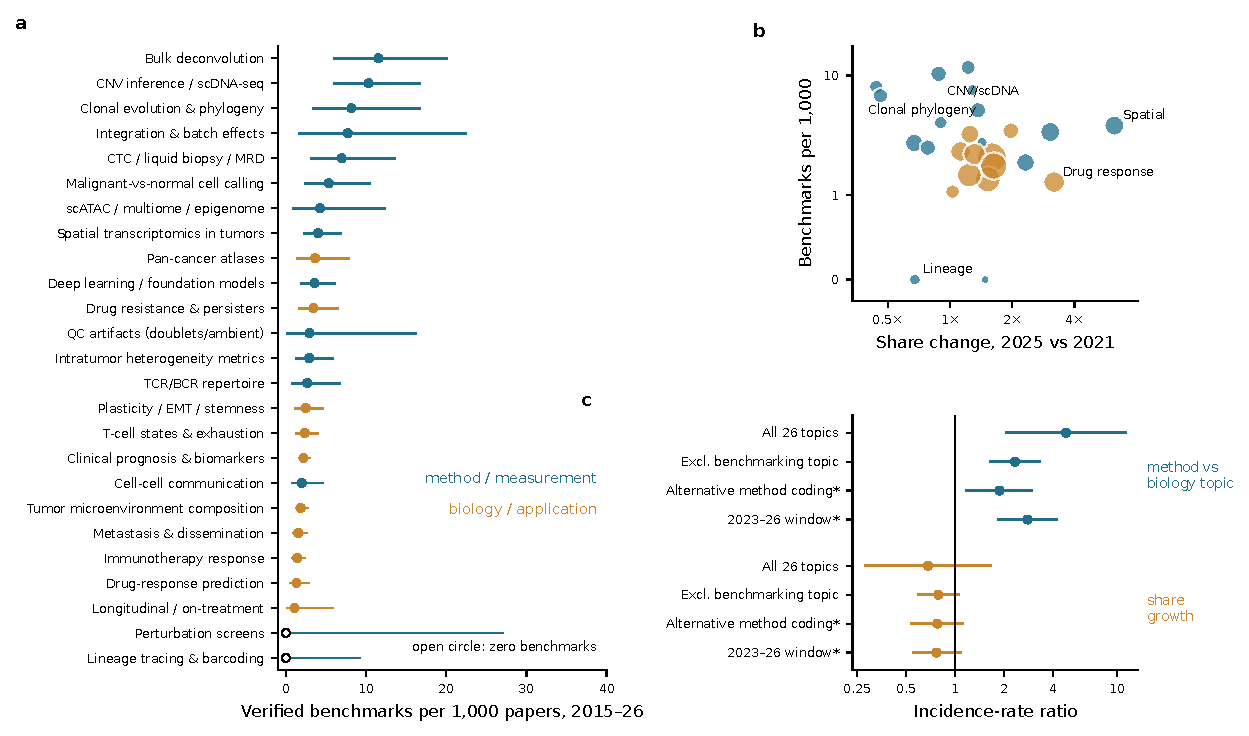
\includegraphics[keepaspectratio,alt={Figure 2. Benchmark
coverage across topics, 2015--2026. (a) Verified benchmarks per 1,000
topic papers, 1 January 2015 to 15 October 2026, with exact Poisson 95\%
intervals; open circles mark the two topics with no benchmark (lineage
tracing, 397 papers; perturbation screens, 136 papers). The benchmarking
topic itself (121 per 1,000) is omitted for scale. (b) Coverage plotted
against share change, 2025 versus 2021; marker area is proportional to
the square root of topic volume, and a 0.3 offset places zero counts on
the log axis. (c) Incidence-rate ratios (IRR) with 95\% CIs from NB2
negative-binomial regressions of topic benchmark counts on topic class
(method versus biology) and log share change, with an offset of log
topic volume. Rows show the full-window fit (n = 26 topics), the fit
excluding the benchmarking topic (n = 25), an alternative topic coding
and the 2023--26 window; * marks fits that exclude the benchmarking
topic. Values greater than 1 indicate more benchmarks per
paper.}]{fig/fig2_coverage.pdf}}
\caption{\textbf{Figure 2. Benchmark coverage across topics,
2015--2026.} (a) Verified benchmarks per 1,000 topic papers, 1 January
2015 to 15 October 2026, with exact Poisson 95\% intervals; open circles
mark the two topics with no benchmark (lineage tracing, 397 papers;
perturbation screens, 136 papers). The benchmarking topic itself (121
per 1,000) is omitted for scale. (b) Coverage plotted against share
change, 2025 versus 2021; marker area is proportional to the square root
of topic volume, and a 0.3 offset places zero counts on the log axis.
(c) Incidence-rate ratios (IRR) with 95\% CIs from NB2 negative-binomial
regressions of topic benchmark counts on topic class (method versus
biology) and log share change, with an offset of log topic volume. Rows
show the full-window fit (n = 26 topics), the fit excluding the
benchmarking topic (n = 25), an alternative topic coding and the
2023--26 window; * marks fits that exclude the benchmarking topic.
Values greater than 1 indicate more benchmarks per paper.}
\end{figure}

\begin{tablefont}

\begin{longtable}[l]{@{}
  >{\raggedright\arraybackslash}p{(\linewidth - 10\tabcolsep) * \real{0.3200}}
  >{\raggedright\arraybackslash}p{(\linewidth - 10\tabcolsep) * \real{0.1200}}
  >{\raggedright\arraybackslash}p{(\linewidth - 10\tabcolsep) * \real{0.1200}}
  >{\raggedright\arraybackslash}p{(\linewidth - 10\tabcolsep) * \real{0.2000}}
  >{\raggedright\arraybackslash}p{(\linewidth - 10\tabcolsep) * \real{0.1200}}
  >{\raggedright\arraybackslash}p{(\linewidth - 10\tabcolsep) * \real{0.1200}}@{}}
\caption{\textbf{Table 2.} Verified benchmark coverage by topic, 2015--2026.
Benchmarks per 1,000 papers use benchmarks and papers published 1
January 2015 to 15 October 2026, with exact Poisson 95\% intervals; the
2023--26 rate is shown for comparison.}\tabularnewline
\toprule
\begin{minipage}[b]{\linewidth}\raggedright
\thead{Topic}
\end{minipage} & \begin{minipage}[b]{\linewidth}\raggedright
\thead{Papers 2015--26}
\end{minipage} & \begin{minipage}[b]{\linewidth}\raggedright
\thead{Benchmarks 2015--26}
\end{minipage} & \begin{minipage}[b]{\linewidth}\raggedright
\thead{Per 1,000 (95\% CI)}
\end{minipage} & \begin{minipage}[b]{\linewidth}\raggedright
\thead{Papers per benchmark}
\end{minipage} & \begin{minipage}[b]{\linewidth}\raggedright
\thead{Per 1,000, 2023--26}
\end{minipage} \\
\midrule
\endfirsthead
\toprule
\begin{minipage}[b]{\linewidth}\raggedright
\thead{Topic}
\end{minipage} & \begin{minipage}[b]{\linewidth}\raggedright
\thead{Papers 2015--26}
\end{minipage} & \begin{minipage}[b]{\linewidth}\raggedright
\thead{Benchmarks 2015--26}
\end{minipage} & \begin{minipage}[b]{\linewidth}\raggedright
\thead{Per 1,000 (95\% CI)}
\end{minipage} & \begin{minipage}[b]{\linewidth}\raggedright
\thead{Papers per benchmark}
\end{minipage} & \begin{minipage}[b]{\linewidth}\raggedright
\thead{Per 1,000, 2023--26}
\end{minipage} \\
\midrule
\endhead
\bottomrule
\endlastfoot
Perturbation screens & 136 & 0 & 0.00 (0.00--27.12) & --- & 0.00 \\
Lineage tracing \& barcoding & 397 & 0 & 0.00 (0.00--9.29) & --- &
0.00 \\
Longitudinal / on-treatment & 930 & 1 & 1.08 (0.03--5.99) & 930 &
0.00 \\
Drug-response prediction & 4,528 & 6 & 1.33 (0.49--2.88) & 755 & 1.28 \\
Immunotherapy response & 9,259 & 13 & 1.40 (0.75--2.40) & 712 & 1.46 \\
Metastasis \& dissemination & 7,811 & 12 & 1.54 (0.79--2.68) & 651 &
1.75 \\
Tumor microenvironment composition & 11,369 & 21 & 1.85 (1.14--2.82) &
541 & 1.71 \\
Cell-cell communication & 2,524 & 5 & 1.98 (0.64--4.62) & 505 & 2.28 \\
Clinical prognosis \& biomarkers & 16,859 & 37 & 2.19 (1.55--3.03) & 456
& 1.70 \\
T-cell states \& exhaustion & 5,127 & 12 & 2.34 (1.21--4.09) & 427 &
2.68 \\
Plasticity / EMT / stemness & 3,653 & 9 & 2.46 (1.13--4.68) & 406 &
0.38 \\
TCR/BCR repertoire & 1,508 & 4 & 2.65 (0.72--6.79) & 377 & 1.94 \\
Intratumor heterogeneity metrics & 2,416 & 7 & 2.90 (1.16--5.97) & 345 &
3.21 \\
QC artifacts (doublets/ambient) & 342 & 1 & 2.92 (0.07--16.29) & 342 &
3.64 \\
Drug resistance \& persisters & 2,624 & 9 & 3.43 (1.57--6.51) & 292 &
2.55 \\
Deep learning / foundation models & 3,361 & 12 & 3.57 (1.84--6.24) & 280
& 3.00 \\
Pan-cancer atlases & 1,643 & 6 & 3.65 (1.34--7.95) & 274 & 4.31 \\
Spatial transcriptomics in tumors & 3,231 & 13 & 4.02 (2.14--6.88) & 249
& 4.29 \\
scATAC / multiome / epigenome & 706 & 3 & 4.25 (0.88--12.42) & 235 &
5.24 \\
Malignant-vs-normal cell calling & 1,500 & 8 & 5.33 (2.30--10.51) & 188
& 4.95 \\
CTC / liquid biopsy / MRD & 1,151 & 8 & 6.95 (3.00--13.70) & 144 &
5.28 \\
Integration \& batch effects & 389 & 3 & 7.71 (1.59--22.54) & 130 &
6.17 \\
Clonal evolution \& phylogeny & 857 & 7 & 8.17 (3.28--16.83) & 122 &
14.96 \\
CNV inference / scDNA-seq & 1,553 & 16 & 10.30 (5.89--16.73) & 97 &
11.48 \\
Bulk deconvolution & 1,040 & 12 & 11.54 (5.96--20.16) & 87 & 11.82 \\
Benchmarking \& evaluation & 373 & 45 & 120.64 (88.00--161.43) & 8 &
123.67 \\
\end{longtable}

\end{tablefont}

\subsection{3.3 What the literature says is wrong, and what survives re-coding}\label{what-the-literature-says-is-wrong-and-what-survives-re-coding}

Under first-pass coding, the most common methodological problem was ``no
ground truth'' (364/1,506; 24.2\%, 22.1--26.4). It was the top-ranked
problem in 21 of 26 topics. It was followed by causality (19.9\%) and
interpretability (12.5\%) (Table 3). Three categories describe checks
that need no gold standard, and all three were rare: parameter
sensitivity (2.3\%, 1.6--3.1), metric invalidity (1.1\%, 0.7--1.7) and
uncertainty (0.7\%, 0.4--1.2).

Independent re-coding changes the interpretation of the most common
category (Fig. 3). Benchmark classification showed substantial
agreement: 88.5\% and κ = 0.74 (0.68--0.80), or κ = 0.76 on the 394
abstracts rated by the model. The second pass found 166 benchmarks
against 158, and the two passes agreed on 134. Problem-type coding
replicated poorly overall (pooled κ = 0.23, 0.17--0.29). ``No ground
truth'' did not replicate at all: 45 of 200 subsample abstracts under
the first pass, 1 under the second (κ = −0.01). The second coder
assigned 30 of the 45 to causality and 9 to interpretability. On
inspection, these statements describe unknown mechanisms or an
uncharacterised landscape rather than the absence of a reference
standard. Merging the three knowledge-gap categories raised agreement to
κ = 0.51 (0.38--0.62). The 24.2\% figure therefore measures the field's
statements of unknown biology, not a stated shortage of evaluation
truth, and we do not use it as evidence of an evaluation deficit.

The three neglected checks behave differently. They are rare under both
codings: in the 200-abstract subsample, metric invalidity was 4 versus
0, parameter sensitivity 2 versus 0, and uncertainty 0 versus 0. Their κ
values are undefined or zero because almost nothing is coded in either
pass. Rarity is the replicated finding; the per-category agreement
statistic is uninformative at this prevalence. We therefore test the
same three checks directly in the benchmark literature (§3.4), where the
question is whether the evaluation was done, not whether authors
complained about its absence.

To test whether these patterns hold across the history of the field, we
coded a stratified sample of abstracts from 2015 to 2026 under explicit
definitions (§2.4; Fig. 4). The 1,800 draws contained 1,771 unique
abstracts, of which 989 used single-cell omics data. Under the explicit
definition, ``no ground truth'' was stated in 1.1\% (0.6--2.0) of these
abstracts, confirming that the first-pass figure of 24.2\% reflected a
loose category rather than a frequent complaint. The most frequently
stated problems were sample size (15.3\% (13.2--17.6)), generalisability
(14.5\% (12.4--16.8)) and clinical translation (8.5\% (6.9--10.4)); the
last increased over time (OR 1.14 per year (1.05--1.24)). The five
problem types that correspond to evaluation checks were each stated in
less than 2\% of abstracts: parameter sensitivity 1.8\% (1.2--2.9),
absence of benchmarks 1.4\% (0.8--2.4), uncertainty 1.3\% (0.8--2.2),
absence of ground truth 1.1\% (0.6--2.0) and metric validity 0.4\%
(0.2--1.0). Taken together, the share of abstracts stating any of the
five fell from 14.0\% in 2015--18 to 3.6\% in 2024--26 (OR 0.81 per
year, 0.74--0.88; Fig. 4c), a steeper decline than for any stated
problem (55.0\% to 41.2\%; OR 0.94 per year (0.90--0.98)). Agreement
between two model coders on 150 abstracts was high for the
single-cell-omics flag (κ = 0.88) and for technical artefacts (κ =
0.85), moderate for sample size (κ = 0.63), and low for the presence of
any stated problem (κ = 0.35) and for most rare categories, which had
five or fewer positives under either coder. Because a single coder and
prompt were applied to every year, systematic coder bias is constant
across years, but the absolute prevalences should be interpreted as
approximate.

\begin{figure}[!htbp]
\centering
\pandocbounded{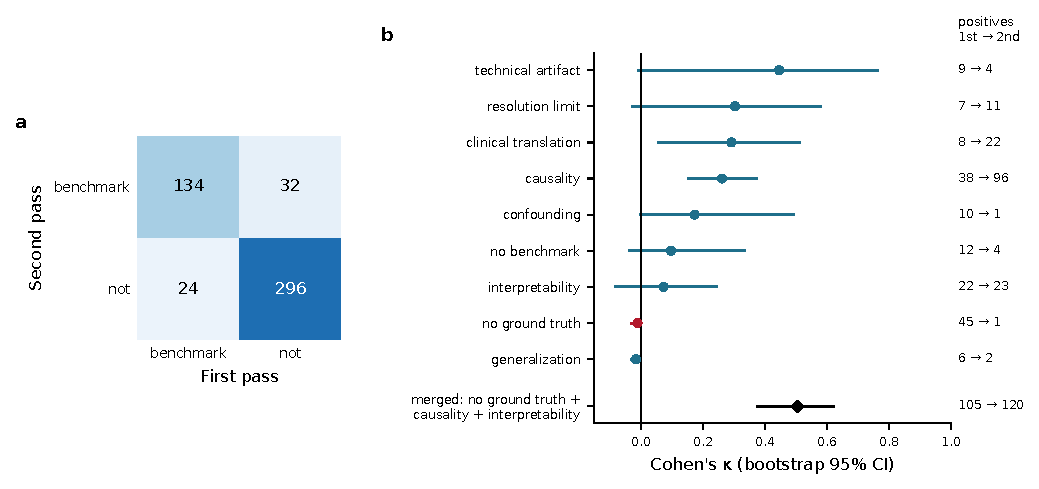
\includegraphics[keepaspectratio,alt={Figure 3.
Reliability of benchmark and problem-type coding. (a) First-pass versus
second-pass classification of the 486 evaluation-titled papers; Cohen's
κ = 0.74 (bootstrap 95\% CI 0.68--0.80), with 88.5\% agreement. (b)
Per-category Cohen's κ (bootstrap 95\% CI) for problem-type coding on a
random subsample of 200 abstracts, for categories with at least five
positives in either pass. Numbers at right give positives under the
first and the second pass. The red marker is ``no ground truth'' (45
versus 1; κ = −0.01). The black diamond merges no ground truth,
causality and interpretability into one knowledge-gap category (κ =
0.51). Categories with almost no positives in either pass (metric
invalidity, parameter sensitivity and uncertainty) are omitted because κ
is undefined or uninformative at that prevalence. Second-pass labels for
92 benchmark abstracts and all 200 problem-type abstracts were produced
by a language-model rater (§2.3).}]{fig/fig4_reliability.pdf}}
\caption{\textbf{Figure 3. Reliability of benchmark and problem-type
coding.} (a) First-pass versus second-pass classification of the 486
evaluation-titled papers; Cohen's κ = 0.74 (bootstrap 95\% CI
0.68--0.80), with 88.5\% agreement. (b) Per-category Cohen's κ
(bootstrap 95\% CI) for problem-type coding on a random subsample of 200
abstracts, for categories with at least five positives in either pass.
Numbers at right give positives under the first and the second pass. The
red marker is ``no ground truth'' (45 versus 1; κ = −0.01). The black
diamond merges no ground truth, causality and interpretability into one
knowledge-gap category (κ = 0.51). Categories with almost no positives
in either pass (metric invalidity, parameter sensitivity and
uncertainty) are omitted because κ is undefined or uninformative at that
prevalence. Second-pass labels for 92 benchmark abstracts and all 200
problem-type abstracts were produced by a language-model rater (§2.3).}
\end{figure}

\begin{figure}[!htbp]
\centering
\pandocbounded{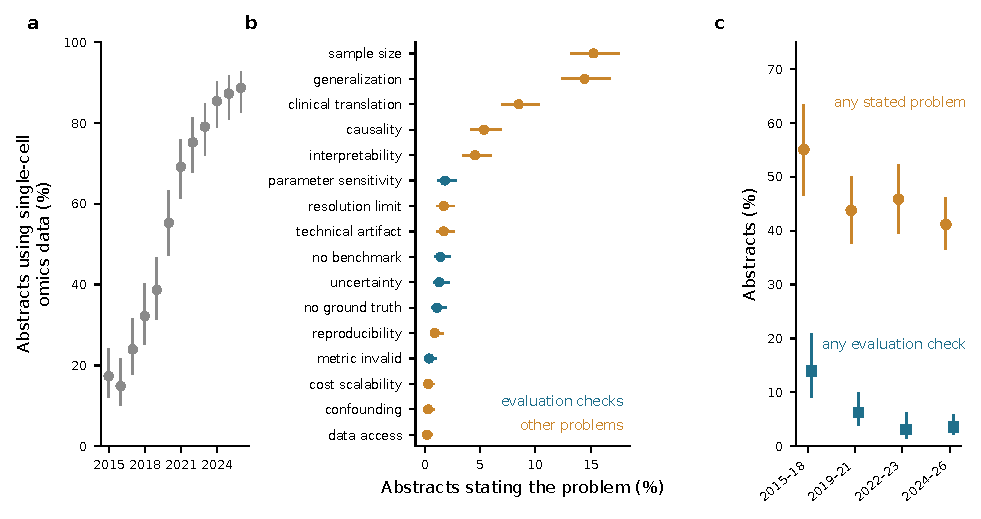
\includegraphics[keepaspectratio,alt={Figure 4. Stated
methodological problems in single-cell cancer abstracts, 2015--2026. A
stratified random sample of 150 research abstracts per year was coded
under explicit definitions (1,771 unique abstracts; 29 papers drawn in
two adjacent years counted once). (a) Percentage of sampled abstracts
that generate or analyse single-cell omics data, by year (Wilson 95\%
CI); the remainder use non-sequencing single-cell assays. (b) Percentage
of the 989 single-cell-omics abstracts stating each problem type (Wilson
95\% CI); blue marks the five types that correspond to evaluation
checks. (c) Percentage of single-cell-omics abstracts stating any
problem (circles) or any evaluation-check problem (squares), by period
(n = 129, 240, 229, 391). The evaluation-check share fell from 14.0\% to
3.6\% (odds ratio 0.81 per year,
0.74--0.88).}]{fig/fig6_problems_time.pdf}}
\caption{\textbf{Figure 4. Stated methodological problems in single-cell
cancer abstracts, 2015--2026.} A stratified random sample of 150
research abstracts per year was coded under explicit definitions (1,771
unique abstracts; 29 papers drawn in two adjacent years counted once).
(a) Percentage of sampled abstracts that generate or analyse single-cell
omics data, by year (Wilson 95\% CI); the remainder use non-sequencing
single-cell assays. (b) Percentage of the 989 single-cell-omics
abstracts stating each problem type (Wilson 95\% CI); blue marks the
five types that correspond to evaluation checks. (c) Percentage of
single-cell-omics abstracts stating any problem (circles) or any
evaluation-check problem (squares), by period (n = 129, 240, 229, 391).
The evaluation-check share fell from 14.0\% to 3.6\% (odds ratio 0.81
per year, 0.74--0.88).}
\end{figure}

\begin{tablefont}

\begin{longtable}[l]{@{}
  >{\raggedright\arraybackslash}p{(\linewidth - 10\tabcolsep) * \real{0.2400}}
  >{\raggedright\arraybackslash}p{(\linewidth - 10\tabcolsep) * \real{0.2000}}
  >{\raggedright\arraybackslash}p{(\linewidth - 10\tabcolsep) * \real{0.0800}}
  >{\raggedright\arraybackslash}p{(\linewidth - 10\tabcolsep) * \real{0.2000}}
  >{\raggedright\arraybackslash}p{(\linewidth - 10\tabcolsep) * \real{0.2000}}
  >{\raggedright\arraybackslash}p{(\linewidth - 10\tabcolsep) * \real{0.0800}}@{}}
\caption{\textbf{Table 3.} Stated methodological problems: archived first-pass
coding (2023--26) and explicit-definition coding (2015--26). Left:
first-pass shares of 1,506 methodological problems (Wilson 95\% CI) and
Cohen's κ against an independent re-coding of 200 abstracts. Right:
percentage of 989 single-cell-omics abstracts (stratified sample,
2015--26) stating each problem under explicit definitions, odds ratio
per year from logistic regression, and κ between two model coders on 150
abstracts. --- indicates undefined or inestimable.}\tabularnewline
\toprule
\begin{minipage}[b]{\linewidth}\raggedright
\thead{Problem type}
\end{minipage} & \begin{minipage}[b]{\linewidth}\raggedright
\thead{First pass \% (95\% CI)}
\end{minipage} & \begin{minipage}[b]{\linewidth}\raggedright
\thead{κ re-code}
\end{minipage} & \begin{minipage}[b]{\linewidth}\raggedright
\thead{2015--26 \% (95\% CI)}
\end{minipage} & \begin{minipage}[b]{\linewidth}\raggedright
\thead{OR per year (95\% CI)}
\end{minipage} & \begin{minipage}[b]{\linewidth}\raggedright
\thead{κ model pair}
\end{minipage} \\
\midrule
\endfirsthead
\toprule
\begin{minipage}[b]{\linewidth}\raggedright
\thead{Problem type}
\end{minipage} & \begin{minipage}[b]{\linewidth}\raggedright
\thead{First pass \% (95\% CI)}
\end{minipage} & \begin{minipage}[b]{\linewidth}\raggedright
\thead{κ re-code}
\end{minipage} & \begin{minipage}[b]{\linewidth}\raggedright
\thead{2015--26 \% (95\% CI)}
\end{minipage} & \begin{minipage}[b]{\linewidth}\raggedright
\thead{OR per year (95\% CI)}
\end{minipage} & \begin{minipage}[b]{\linewidth}\raggedright
\thead{κ model pair}
\end{minipage} \\
\midrule
\endhead
\bottomrule
\endlastfoot
no ground truth & 24.2 (22.1--26.4) & -0.01 & 1.1 (0.6--2.0) & 0.70
(0.57--0.85) & -0.01 \\
causality & 19.9 (17.9--21.9) & 0.26 & 5.4 (4.1--6.9) & 1.01
(0.92--1.11) & 0.38 \\
interpretability & 12.5 (11.0--14.3) & 0.07 & 4.6 (3.4--6.0) & 0.88
(0.80--0.96) & 0.25 \\
other & 6.4 (5.2--7.7) & -0.05 & 0.1 (0.0--0.6) & --- & 0.00 \\
no benchmark & 5.8 (4.7--7.1) & 0.10 & 1.4 (0.8--2.4) & 0.82
(0.70--0.97) & --- \\
generalization & 5.7 (4.6--7.0) & -0.01 & 14.5 (12.4--16.8) & 0.99
(0.93--1.05) & 0.13 \\
resolution limit & 5.6 (4.5--6.9) & 0.30 & 1.7 (1.1--2.7) & 0.70
(0.60--0.82) & 0.39 \\
technical artifact & 5.2 (4.2--6.4) & 0.45 & 1.7 (1.1--2.7) & 0.80
(0.69--0.93) & 0.85 \\
confounding & 3.3 (2.5--4.4) & 0.17 & 0.3 (0.1--0.9) & 0.82 (0.58--1.17)
& 0.00 \\
clinical translation & 3.1 (2.3--4.1) & 0.29 & 8.5 (6.9--10.4) & 1.14
(1.05--1.24) & 0.03 \\
parameter sensitivity & 2.3 (1.6--3.1) & 0.00 & 1.8 (1.2--2.9) & 0.78
(0.67--0.91) & 0.66 \\
sample size & 1.5 (1.0--2.2) & 0.00 & 15.3 (13.2--17.6) & 0.96
(0.90--1.01) & 0.63 \\
cost scalability & 1.3 (0.9--2.0) & -0.01 & 0.3 (0.1--0.9) & 1.33
(0.77--2.28) & 0.00 \\
metric invalid & 1.1 (0.7--1.7) & 0.00 & 0.4 (0.2--1.0) & 1.20
(0.80--1.81) & 0.00 \\
data access & 0.9 (0.6--1.6) & 0.66 & 0.2 (0.1--0.7) & 0.84 (0.54--1.29)
& 0.00 \\
reproducibility & 0.7 (0.4--1.3) & 0.80 & 0.9 (0.5--1.7) & 0.83
(0.68--1.02) & 0.00 \\
uncertainty & 0.7 (0.4--1.2) & --- & 1.3 (0.8--2.2) & 0.93 (0.78--1.11)
& 0.00 \\
\end{longtable}

\end{tablefont}

\subsection{3.4 What benchmarks check}\label{what-benchmarks-check}

The 269 catalogued benchmarks span 16 method classes (Table 4). 151
(56.1\%) were published in 2024--2026 and 48 (17.8\%) are
cancer-specific. Simulation was the most commonly stated source of
ground truth (91; 33.8\%). Orthogonal assays were stated in 44 (16.4\%)
and expert or published labels in 24 (8.9\%). Held-out experimental
measurements appeared in 12, genotype multiplexing in 11 and cell-line
mixtures in 8. 107 abstracts (39.8\%) did not state their ground truth
at all (Fig. 5a).

Physical ground truth is concentrated in a few classes. Doublet and
ambient-RNA benchmarks use genotype or synthetic-barcode truth in 10 of
13. Perturbation-prediction benchmarks score held-out measurements in 10
of 11. Annotation benchmarks rely on expert labels in 9 of 17, and
foundation-model evaluations do not state truth in 11 of 14.

Robustness to parameters or pipeline choices was stated in 15 benchmarks
(5.6\%), calibration or uncertainty in 9 (3.3\%) and metric validity in
8 (3.0\%) (Fig. 5b). Among the 48 cancer-specific benchmarks the counts
were 4, 2 and 0. Abstract-level coding undercounts these checks. Even
so, the same three dimensions are the least represented both in what the
literature states as problems and in what the benchmarks report doing.
This convergence, from two independent sources, is the central empirical
result of this review.

\begin{figure}[!htbp]
\centering
\pandocbounded{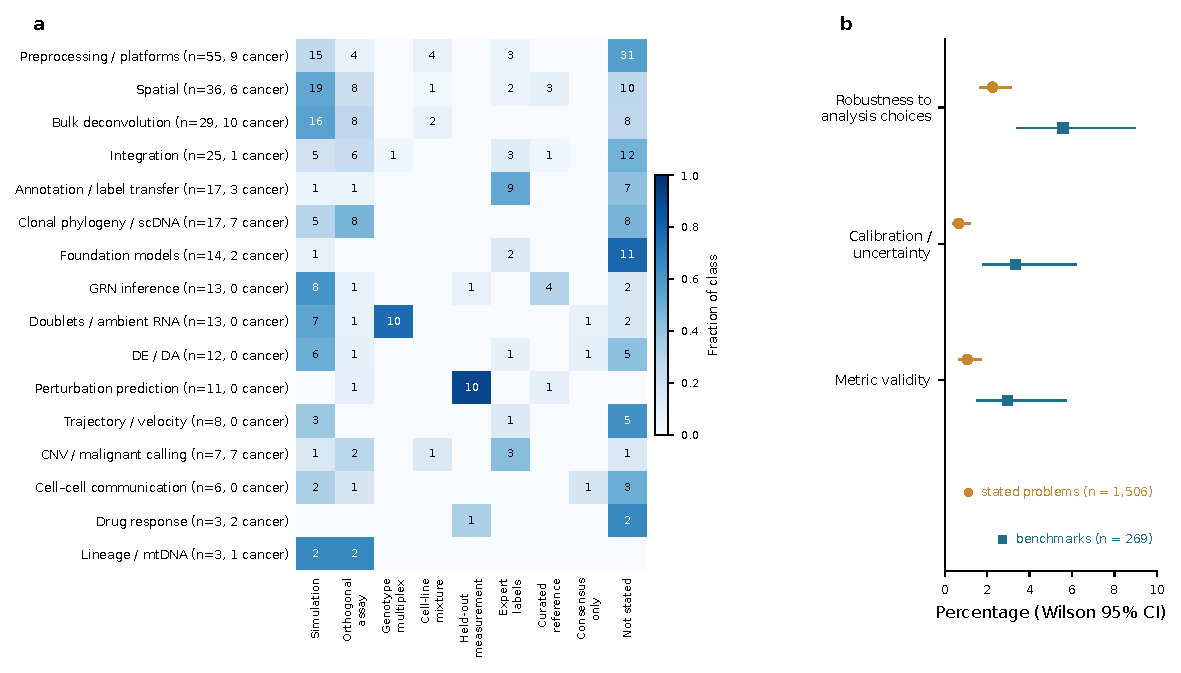
\includegraphics[keepaspectratio,alt={Figure 5.
Ground-truth strategies and reported checks in 269 benchmark studies.
(a) Stated ground-truth strategy by method class. Cell values are counts
and shading gives the fraction of benchmarks in the class; a benchmark
may state more than one strategy. Row labels give class size and the
number of cancer-specific benchmarks. Simulation is the most frequent
stated strategy (91 of 269); 107 abstracts state none. (b) Percentage of
benchmarks whose abstract reports an assessment of robustness to
analytical choices (15), calibration or uncertainty (9) or metric
validity (8) (squares; n = 269). Circles show the share of the
corresponding categories among 1,506 first-pass stated methodological
problems (34, 10 and 16). Intervals are Wilson 95\% CIs. Because coding
used abstracts, all values are lower bounds.}]{fig/fig3_practice.pdf}}
\caption{\textbf{Figure 5. Ground-truth strategies and reported checks
in 269 benchmark studies.} (a) Stated ground-truth strategy by method
class. Cell values are counts and shading gives the fraction of
benchmarks in the class; a benchmark may state more than one strategy.
Row labels give class size and the number of cancer-specific benchmarks.
Simulation is the most frequent stated strategy (91 of 269); 107
abstracts state none. (b) Percentage of benchmarks whose abstract
reports an assessment of robustness to analytical choices (15),
calibration or uncertainty (9) or metric validity (8) (squares; n =
269). Circles show the share of the corresponding categories among 1,506
first-pass stated methodological problems (34, 10 and 16). Intervals are
Wilson 95\% CIs. Because coding used abstracts, all values are lower
bounds.}
\end{figure}

\begin{tablefont}

\setlength{\tabcolsep}{2pt}
\begin{longtable}[l]{@{}
  >{\raggedright\arraybackslash}p{(\linewidth - 26\tabcolsep) * \real{0.1350}}
  >{\raggedright\arraybackslash}p{(\linewidth - 26\tabcolsep) * \real{0.0300}}
  >{\raggedright\arraybackslash}p{(\linewidth - 26\tabcolsep) * \real{0.0650}}
  >{\raggedright\arraybackslash}p{(\linewidth - 26\tabcolsep) * \real{0.1000}}
  >{\raggedright\arraybackslash}p{(\linewidth - 26\tabcolsep) * \real{0.0660}}
  >{\raggedright\arraybackslash}p{(\linewidth - 26\tabcolsep) * \real{0.0660}}
  >{\raggedright\arraybackslash}p{(\linewidth - 26\tabcolsep) * \real{0.0660}}
  >{\raggedright\arraybackslash}p{(\linewidth - 26\tabcolsep) * \real{0.0660}}
  >{\raggedright\arraybackslash}p{(\linewidth - 26\tabcolsep) * \real{0.0660}}
  >{\raggedright\arraybackslash}p{(\linewidth - 26\tabcolsep) * \real{0.0660}}
  >{\raggedright\arraybackslash}p{(\linewidth - 26\tabcolsep) * \real{0.0660}}
  >{\raggedright\arraybackslash}p{(\linewidth - 26\tabcolsep) * \real{0.0660}}
  >{\raggedright\arraybackslash}p{(\linewidth - 26\tabcolsep) * \real{0.0660}}
  >{\raggedright\arraybackslash}p{(\linewidth - 26\tabcolsep) * \real{0.0660}}@{}}
\caption{\textbf{Table 4.} Benchmark catalogue by method class. Counts of
benchmarks whose abstract states each ground-truth strategy or
assessment (lower bounds). Sim., simulation; Orth., orthogonal assay;
Geno., genotype multiplexing; Mix., cell-line mixture; Held-out,
held-out experimental measurements; Expert, expert or published labels;
Robust., robustness to parameters; Calib., calibration/uncertainty;
Metric, metric validity.}\tabularnewline
\toprule
\begin{minipage}[b]{\linewidth}\raggedright
\thead{Class}
\end{minipage} & \begin{minipage}[b]{\linewidth}\raggedright
\thead{n}
\end{minipage} & \begin{minipage}[b]{\linewidth}\raggedright
\thead{Cancer}
\end{minipage} & \begin{minipage}[b]{\linewidth}\raggedright
\thead{Years}
\end{minipage} & \begin{minipage}[b]{\linewidth}\raggedright
\thead{Sim.}
\end{minipage} & \begin{minipage}[b]{\linewidth}\raggedright
\thead{Orth.}
\end{minipage} & \begin{minipage}[b]{\linewidth}\raggedright
\thead{Geno.}
\end{minipage} & \begin{minipage}[b]{\linewidth}\raggedright
\thead{Mix.}
\end{minipage} & \begin{minipage}[b]{\linewidth}\raggedright
\thead{Held-out}
\end{minipage} & \begin{minipage}[b]{\linewidth}\raggedright
\thead{Expert}
\end{minipage} & \begin{minipage}[b]{\linewidth}\raggedright
\thead{Not stated}
\end{minipage} & \begin{minipage}[b]{\linewidth}\raggedright
\thead{Robust.}
\end{minipage} & \begin{minipage}[b]{\linewidth}\raggedright
\thead{Calib.}
\end{minipage} & \begin{minipage}[b]{\linewidth}\raggedright
\thead{Metric}
\end{minipage} \\
\midrule
\endfirsthead
\toprule
\begin{minipage}[b]{\linewidth}\raggedright
\thead{Class}
\end{minipage} & \begin{minipage}[b]{\linewidth}\raggedright
\thead{n}
\end{minipage} & \begin{minipage}[b]{\linewidth}\raggedright
\thead{Cancer}
\end{minipage} & \begin{minipage}[b]{\linewidth}\raggedright
\thead{Years}
\end{minipage} & \begin{minipage}[b]{\linewidth}\raggedright
\thead{Sim.}
\end{minipage} & \begin{minipage}[b]{\linewidth}\raggedright
\thead{Orth.}
\end{minipage} & \begin{minipage}[b]{\linewidth}\raggedright
\thead{Geno.}
\end{minipage} & \begin{minipage}[b]{\linewidth}\raggedright
\thead{Mix.}
\end{minipage} & \begin{minipage}[b]{\linewidth}\raggedright
\thead{Held-out}
\end{minipage} & \begin{minipage}[b]{\linewidth}\raggedright
\thead{Expert}
\end{minipage} & \begin{minipage}[b]{\linewidth}\raggedright
\thead{Not stated}
\end{minipage} & \begin{minipage}[b]{\linewidth}\raggedright
\thead{Robust.}
\end{minipage} & \begin{minipage}[b]{\linewidth}\raggedright
\thead{Calib.}
\end{minipage} & \begin{minipage}[b]{\linewidth}\raggedright
\thead{Metric}
\end{minipage} \\
\midrule
\endhead
\bottomrule
\endlastfoot
Preprocessing / platforms & 55 & 9 & 2018-2026 & 15 & 4 & 0 & 4 & 0 & 3
& 31 & 3 & 1 & 1 \\
Spatial & 36 & 6 & 2022-2026 & 19 & 8 & 0 & 1 & 0 & 2 & 10 & 1 & 2 &
1 \\
Bulk deconvolution & 29 & 10 & 2019-2026 & 16 & 8 & 0 & 2 & 0 & 0 & 8 &
1 & 0 & 0 \\
Integration & 25 & 1 & 2019-2026 & 5 & 6 & 1 & 0 & 0 & 3 & 12 & 1 & 0 &
1 \\
Annotation / label transfer & 17 & 3 & 2019-2026 & 1 & 1 & 0 & 0 & 0 & 9
& 7 & 0 & 0 & 0 \\
Clonal phylogeny / scDNA & 17 & 7 & 2006-2025 & 5 & 8 & 0 & 0 & 0 & 0 &
8 & 1 & 0 & 0 \\
Foundation models & 14 & 2 & 2024-2026 & 1 & 0 & 0 & 0 & 0 & 2 & 11 & 1
& 0 & 0 \\
GRN inference & 13 & 0 & 2018-2026 & 8 & 1 & 0 & 0 & 1 & 0 & 2 & 0 & 1 &
1 \\
Doublets / ambient RNA & 13 & 0 & 2021-2026 & 7 & 1 & 10 & 0 & 0 & 0 & 2
& 1 & 0 & 0 \\
DE / DA & 12 & 0 & 2017-2024 & 6 & 1 & 0 & 0 & 0 & 1 & 5 & 2 & 4 & 0 \\
Perturbation prediction & 11 & 0 & 2025-2026 & 0 & 1 & 0 & 0 & 10 & 0 &
0 & 1 & 1 & 4 \\
Trajectory / velocity & 8 & 0 & 2019-2026 & 3 & 0 & 0 & 0 & 0 & 1 & 5 &
0 & 0 & 0 \\
CNV / malignant calling & 7 & 7 & 2024-2026 & 1 & 2 & 0 & 1 & 0 & 3 & 1
& 3 & 0 & 0 \\
Cell--cell communication & 6 & 0 & 2022-2026 & 2 & 1 & 0 & 0 & 0 & 0 & 3
& 0 & 0 & 0 \\
Drug response & 3 & 2 & 2025-2026 & 0 & 0 & 0 & 0 & 1 & 0 & 2 & 0 & 0 &
0 \\
Lineage / mtDNA & 3 & 1 & 2021-2026 & 2 & 2 & 0 & 0 & 0 & 0 & 0 & 0 & 0
& 0 \\
\end{longtable}

\end{tablefont}

\section{4. State of evaluation by method class}\label{state-of-evaluation-by-method-class}

This section summarises, for each method class, the findings that are
consistent across benchmarks, those that conflict, and the questions
that no benchmark has addressed. Counts refer to the 269-record
catalogue (Supplementary Data S1); claims are limited to what the cited
abstracts report.

\subsection{4.1 CNV inference and malignant-cell calling}\label{cnv-inference-and-malignant-cell-calling}

All seven benchmarks in this class are cancer-specific and published in
2024--2026 {[}26--31{]}. A consensus is emerging but conditional.
Haplotype-aware inference with Numbat {[}24{]} leads when allelic
information is available. Expression-only callers such as copyKAT
{[}23{]} and SCEVAN {[}32{]} are the practical default otherwise, though
inferCNV-style smoothing {[}20,21{]} remains the most used. Two
disease-specific comparisons found less than 30\% overlap between
callers and many false positives {[}28,29{]}. Reference choice, depth
and purity change results {[}26,27{]}. This is the only class in which
sensitivity to the reference is routinely reported. No benchmark scores
the binary malignant call against a shared, matched DNA-level truth
across tumour types, or stratifies by aneuploidy burden. Near-diploid
tumours, in which expression-based CNV inference has little copy-number
signal to exploit, are not analysed as a separate stratum in any of the
seven benchmarks.

\subsection{4.2 Bulk deconvolution}\label{bulk-deconvolution}

Deconvolution is among the most benchmarked classes, with 29 records, 10
of them cancer-specific. Its ground truth is mostly pseudo-bulk
simulation (16 of 29). Results are sensitive to normalisation and
reference construction {[}18{]} and degrade sharply when a cell type is
missing from the reference {[}18{]}. More realistic heterogeneous
pseudo-bulk reorders the methods {[}33{]}. None of the 29 abstracts
reports uncertainty on estimated proportions, and none examines metric
validity. For tumours, deconvolution of malignant states against
DNA-level truth is missing. The ground-truth catalogue lists 459 series
with paired bulk and single-cell data from the same tumours that could
anchor such a test.

\subsection{4.3 Integration and batch correction}\label{integration-and-batch-correction}

Atlas-level integration has a mature benchmark {[}14{]}, earlier
comparisons {[}13{]} and the only dedicated metric critique in the
catalogue. That critique shows that silhouette-based scores cannot
reliably assess batch removal or conservation of biological signal
{[}34{]}. Only 1 of 25 integration benchmarks is cancer-specific.
Integration benchmarks score the removal of batch effects jointly with
the conservation of biological variation {[}14{]}. In tumours,
patient-specific malignant programmes {[}21,22{]} are confounded with
patient as a batch variable. No integration benchmark in the catalogue
quantifies how much of that patient-specific malignant signal is
removed.

\subsection{4.4 Annotation and label transfer}\label{annotation-and-label-transfer}

General-purpose classifiers are a strong baseline for automatic
annotation {[}12{]}. Annotation benchmarks rely mostly on
author-supplied labels (9 of 17), which raises a circularity problem:
the labels were usually derived from the same marker genes that the
evaluated tools use. Calibration of label confidence and rejection of
unknown cell types are assessed in only one record, and it is not
cancer-specific {[}35{]}. Conformal prediction sets for annotation with
guaranteed coverage have been proposed {[}36{]}, but have not been
evaluated on tumour data. Whether confidence scores remain calibrated
when the malignant compartment is absent from the reference, the default
situation in tumour data, has not been tested.

\subsection{4.5 Cell--cell communication}\label{cellcell-communication}

Communication inference is shaped as much by the choice of
ligand--receptor resource as by the choice of method {[}16{]}. Only 6
benchmarks exist and none is cancer-specific, although communication is
among the fastest-growing topics (2.3-fold share gain). Spatial
co-localisation is used as a proxy truth {[}16,37{]}. No benchmark uses
matched spatial data from the same tumour as an external referee, though
the ground-truth catalogue lists 250 series with paired spatial data.

\subsection{4.6 Spatial transcriptomics}\label{spatial-transcriptomics}

Spatial methods have 36 benchmarks. For spot deconvolution,
cell2location and RCTD are repeatedly among the best {[}17,38{]}, but a
simple regression baseline outperforms nearly half of the dedicated
methods {[}38{]}. No domain-detection method wins across platforms
{[}39{]}. Metric validity is beginning to be examined in this class,
with critiques of spatial ARI {[}40{]} and of clustering-benchmark
pitfalls {[}41{]}. A type-I-error assessment of co-localisation
statistics in cancer {[}42{]} is one of only two calibration analyses
among cancer-specific benchmarks.

\subsection{4.7 Gene-regulatory-network inference}\label{gene-regulatory-network-inference}

GRN benchmarks report modest performance overall. On experimental data,
methods often do not beat random predictors {[}43,44{]}, and
interventional methods do not beat observational ones {[}45{]}. None of
the 13 GRN benchmarks is cancer-specific. The aneuploid tumour genome,
where expression changes track copy number, breaks assumptions that GRN
inference makes in normal tissue, and this has not been benchmarked.

\subsection{4.8 Lineage tracing and clonal phylogeny}\label{lineage-tracing-and-clonal-phylogeny}

Lineage tracing is the thinnest class: 3 records, none of which
benchmarks mitochondrial-variant clone callers. Natural mtDNA mutations
are now an established lineage marker in human cells {[}46--49{]}, and
dedicated variant-selection tools exist {[}50{]}. Yet 266
lineage-tracing papers in 2023--26 rely on these callers without a
neutral comparison. Clonal-phylogeny benchmarks are mostly older
comparisons of whole-genome amplification protocols. No neutral
benchmark of single-cell phylogeny-inference tools on shared truth was
found.

\subsection{4.9 Differential expression and abundance}\label{differential-expression-and-abundance}

DE has the most consistent methodological consensus in the catalogue.
Tests that treat cells as independent replicates inflate false
discoveries, while pseudobulk and mixed models control them
{[}10,51,52{]}. This is the single-cell form of a classical
pseudoreplication error {[}53{]}. DE is also the class in which
calibration (FDR control) is most often assessed (4 of 12). No DE or DA
benchmark is cancer-specific. In tumours, patient-specific malignant
states violate the assumption that cell types are shared across
conditions.

\subsection{4.10 Doublets, demultiplexing and ambient RNA}\label{doublets-demultiplexing-and-ambient-rna}

This is the best-grounded class. Genotype multiplexing {[}54--56{]} and
antibody or lipid hashing {[}57--59{]} supply truth in 10 of 13
benchmarks {[}15,60{]}. None of the 13 is cancer-specific. Because
doublet and ambient-RNA correction precede malignant-cell calling
(§4.1), errors at this step propagate to it, but that propagation has
not been measured in tumour data. Genetic demultiplexing has been shown
to work in pooled tumour samples {[}61{]}, so the experimental design
for a tumour-specific benchmark exists.

\subsection{4.11 Perturbation prediction and foundation models}\label{perturbation-prediction-and-foundation-models}

Perturbation prediction has the strongest consensus in the catalogue.
Simple linear or mean baselines match or beat deep-learning and
foundation-model predictors {[}19,62{]}. It is also the class where
metric validity is most actively studied (4 of 11 records).
Correlation-based scores can be inflated by reusing control cells
{[}63{]}, and R² can hide failures on differentially expressed genes
{[}64{]}. Foundation models do not consistently beat simpler baselines
in zero-shot evaluation {[}65{]}, and show limited advantage for cancer
patient outcomes {[}66{]}. None of these abstracts states a check for
leakage between pretraining corpora and test sets.

\subsection{4.12 Drug-response prediction}\label{drug-response-prediction}

Drug-response prediction gained share 3.2-fold since 2021 but has 3
benchmarks in the catalogue {[}67{]}. No shared single-cell truth set
with measured per-cell or per-clone response exists. Pooled cell-line
designs with SNP demultiplexing {[}68{]} and patient-model
Perturb-CITE-seq {[}69{]} show how one could be built.

\section{5. Three neglected checks}\label{three-neglected-checks}

The analyses in §3 identify three checks that are rare both as stated
problems and as reported analyses. None of them requires a new gold
standard.

\subsection{5.1 Is the metric measuring what it claims?}\label{is-the-metric-measuring-what-it-claims}

A benchmark is only as informative as its scoring function.
Chance-corrected partition agreement {[}70{]} has known dependence on
cluster number and balance {[}71{]}. Silhouette widths {[}72{]} can
reward over-correction in integration {[}34{]}. Two-dimensional
embeddings distort high-dimensional structure in ways that make them
poor evaluation targets {[}73{]}. In perturbation prediction, the choice
of metric and control can change the ranking of methods {[}63,64{]}.
Metric validity can be checked without ground truth. A valid metric must
respond monotonically to controlled degradation (adding noise, merging
clusters, permuting labels). It must not be maximised by trivial
baselines, and it must rank methods consistently with an orthogonal
criterion where one exists. Not one of the 48 cancer-specific benchmarks
in the catalogue reports such a check in its abstract.

\subsection{5.2 Is the conclusion robust to defensible analytical choices?}\label{is-the-conclusion-robust-to-defensible-analytical-choices}

Outside genomics, analytical flexibility is a documented source of false
or fragile findings {[}74,75{]}. Two remedies exist. Multiverse analysis
{[}76{]} and specification-curve analysis {[}77{]} report a result
across all defensible pipelines. Many-analyst studies show directly that
teams given the same data reach different conclusions {[}78,79{]}. A
standard single-cell workflow involves a sequence of defensible but
consequential analytical choices. Transformation choice {[}80{]},
preprocessing pipeline {[}81--83{]} and preprocessing for RNA velocity
{[}84{]} each change downstream results. A recent study of cancer
scRNA-seq reports that normalisation choice alone drives biological
interpretation {[}85{]}. Yet robustness was stated in 5.6\% of
benchmarks and in 4 of 48 cancer-specific ones. The parallel question
for biological claims has not been asked systematically: how often does
the headline result of a tumour scRNA-seq paper survive the defensible
alternatives? Community best-practice guides {[}86,87{]} narrow the
range of choices but do not quantify the sensitivity of conclusions to
the choices that remain.

\subsection{5.3 Is the stated confidence honest?}\label{is-the-stated-confidence-honest}

Modern predictive models are often overconfident {[}88{]}. Conformal
prediction provides distribution-free coverage guarantees for any model
{[}89--91{]}. Single-cell applications are only beginning to appear, for
cell-type annotation {[}36{]} and in the recognition that
reference-based annotation needs explicit uncertainty {[}92{]}.
Calibration was stated in 3.3\% of benchmarks. Per-cell malignancy
probabilities, deconvolution proportions, annotation scores, inferred
interactions and perturbation predictions are almost never reported with
calibrated uncertainty. The relevant test is simple: a reliability
diagram and an expected calibration error against an independent label.
Its most informative stress case is the tumour-specific one, cells from
populations absent from the reference.

\subsection{5.4 Null models}\label{null-models}

A fourth, related check is comparison against an appropriate null. Most
random gene-expression signatures are significantly associated with
breast-cancer outcome {[}93{]}. Meta-analysis of published
ovarian-cancer signatures found modest, overlapping performance across
validation cohorts {[}94{]}. Clinical prognosis is the largest topic in
this subfield (13,532 papers in 2023--26) and produced 23 benchmarks in
that window. Single-cell-derived prognostic signatures have not been
systematically tested against size- and proliferation-matched random
sets.

\section{6. Ground truth already exists}\label{ground-truth-already-exists}

\subsection{6.1 Designs that supply truth}\label{designs-that-supply-truth}

Several experimental designs provide truth independent of the
transcriptome being analysed (Table 5). Cell-line mixtures with known
composition {[}95--98{]} supply known identity and proportions. Genotype
multiplexing with demuxlet, souporcell and vireo {[}54--56{]} and
antibody or lipid hashing {[}57,58{]} supply known sample of origin and
doublet status. Genotype demultiplexing works in pooled tumour samples
{[}61{]}. CITE-seq and related assays {[}99--102{]} give a protein
readout that is measured independently of the RNA used for annotation.
Spike-ins {[}103--105{]} supply known molecule counts. Somatic mtDNA
variants supply lineage relationships {[}46--48{]}. Pooled CRISPR
screens with single-cell readout {[}69,106--108{]} supply known
interventions. Matched exome or genome sequencing supplies DNA-level
truth for malignancy and clone structure.

Simulation remains the most common stated ground truth (33.8\% of
benchmarks), but its fidelity is limited. Most scRNA-seq simulators fail
to reproduce multi-group and batch structure {[}109,110{]}. Newer
simulators improve fidelity {[}111--113{]}, but a ranking obtained on
simulated data needs confirmation on physical truth.

\subsection{6.2 Where it is, publicly}\label{where-it-is-publicly}

The ground-truth catalogue locates 1,336 GEO series (1,166 study groups)
of human tumour single-cell data with at least one orthogonal validation
modality (Fig. 6; Table 5). The modalities are paired bulk RNA in 459
series, longitudinal or on-treatment sampling in 297, paired spatial
data in 250, CITE-seq protein in 227, genotype or hashtag multiplexing
in 166, matched WES/WGS in 138, Perturb-seq in 89, cell-line mixtures in
25 and mtDNA lineage in 18. Three quarters of these series (75.7\%) were
deposited in 2023--26, so the resource is newer than most of the
benchmarks that could use it. Coverage is uneven. Lung cancer is
represented by 19--50 series in each of the six most frequent
modalities, and breast cancer and glioma by 8--47. Cell-line mixtures
and mtDNA lineage data are rare everywhere: 25 and 18 series, with mtDNA
lineage concentrated in chronic lymphocytic leukaemia and colorectal
cancer. Mapping modalities to tasks gives 162 series usable for
malignant-calling truth, 153 for clone calling, 356 for annotation
calibration and 250 for a spatial referee of communication inference.
These complement curated atlases and portals {[}22,25,114--121{]}, which
index expression data but not the validation modalities that make data
usable for evaluation.

\begin{figure}[!htbp]
\centering
\pandocbounded{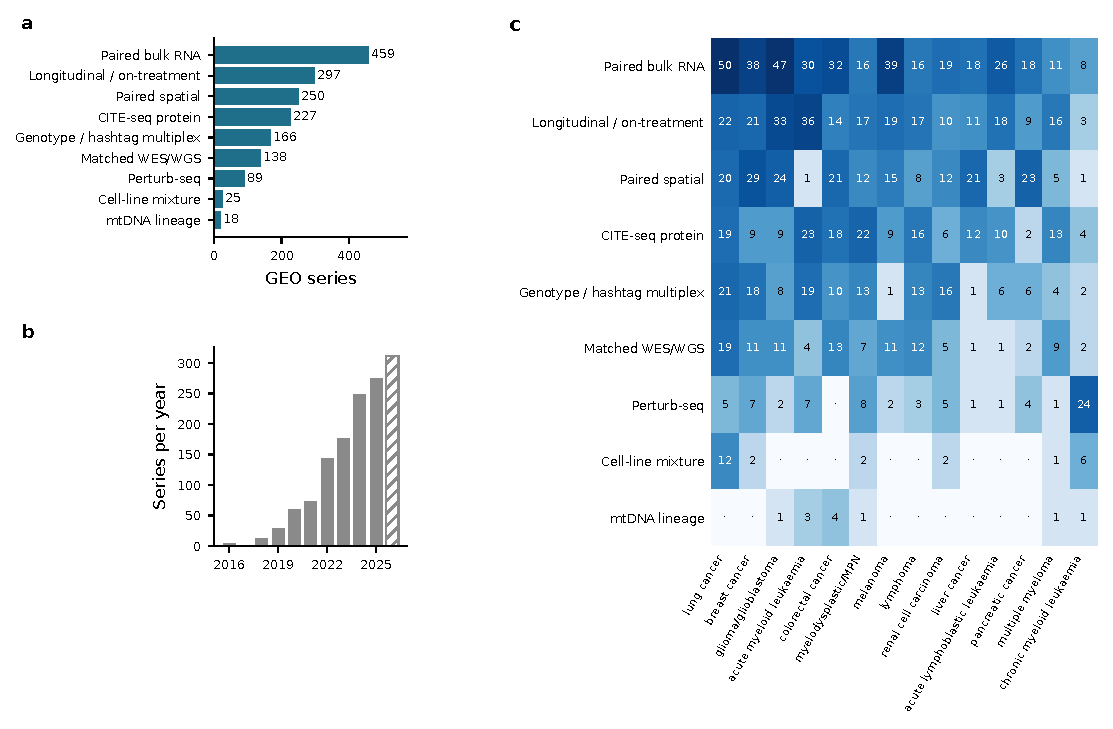
\includegraphics[keepaspectratio,alt={Figure 6. Public
ground truth for evaluating tumour single-cell methods. (a) Number of
GEO series of human tumour single-cell data carrying each orthogonal
validation modality (n = 1,336 series in 1,166 study groups; a series
can carry several modalities). (b) Validation-bearing series by year of
deposition; 75.7\% were deposited in 2023--26, and the hatched 2026 bar
is partial. (c) Series by modality for the 14 most frequent cancer
types; dots indicate zero. Chronic myeloid leukaemia counts are
dominated by K562 Perturb-seq screens. Modality calls were derived from
series-level text with spot-audited regular-expression rules; recall was
not measured, and deposition of controlled-access data was not
verified.}]{fig/fig5_ground_truth.pdf}}
\caption{\textbf{Figure 6. Public ground truth for evaluating tumour
single-cell methods.} (a) Number of GEO series of human tumour
single-cell data carrying each orthogonal validation modality (n = 1,336
series in 1,166 study groups; a series can carry several modalities).
(b) Validation-bearing series by year of deposition; 75.7\% were
deposited in 2023--26, and the hatched 2026 bar is partial. (c) Series
by modality for the 14 most frequent cancer types; dots indicate zero.
Chronic myeloid leukaemia counts are dominated by K562 Perturb-seq
screens. Modality calls were derived from series-level text with
spot-audited regular-expression rules; recall was not measured, and
deposition of controlled-access data was not verified.}
\end{figure}

\begin{tablefont}

\begin{longtable}[l]{@{}
  >{\raggedright\arraybackslash}p{(\linewidth - 10\tabcolsep) * \real{0.1786}}
  >{\raggedright\arraybackslash}p{(\linewidth - 10\tabcolsep) * \real{0.0714}}
  >{\raggedright\arraybackslash}p{(\linewidth - 10\tabcolsep) * \real{0.0714}}
  >{\raggedright\arraybackslash}p{(\linewidth - 10\tabcolsep) * \real{0.0714}}
  >{\raggedright\arraybackslash}p{(\linewidth - 10\tabcolsep) * \real{0.3214}}
  >{\raggedright\arraybackslash}p{(\linewidth - 10\tabcolsep) * \real{0.2857}}@{}}
\caption{\textbf{Table 5.} Public validation-bearing tumour single-cell series in
GEO, by modality. Study groups collapse SuperSeries and their SubSeries.
Tasks are those the modality can supply truth for.}\tabularnewline
\toprule
\begin{minipage}[b]{\linewidth}\raggedright
\thead{Modality}
\end{minipage} & \begin{minipage}[b]{\linewidth}\raggedright
\thead{Series}
\end{minipage} & \begin{minipage}[b]{\linewidth}\raggedright
\thead{Study groups}
\end{minipage} & \begin{minipage}[b]{\linewidth}\raggedright
\thead{Median samples}
\end{minipage} & \begin{minipage}[b]{\linewidth}\raggedright
\thead{Most frequent cancer types (series)}
\end{minipage} & \begin{minipage}[b]{\linewidth}\raggedright
\thead{Benchmark tasks enabled}
\end{minipage} \\
\midrule
\endfirsthead
\toprule
\begin{minipage}[b]{\linewidth}\raggedright
\thead{Modality}
\end{minipage} & \begin{minipage}[b]{\linewidth}\raggedright
\thead{Series}
\end{minipage} & \begin{minipage}[b]{\linewidth}\raggedright
\thead{Study groups}
\end{minipage} & \begin{minipage}[b]{\linewidth}\raggedright
\thead{Median samples}
\end{minipage} & \begin{minipage}[b]{\linewidth}\raggedright
\thead{Most frequent cancer types (series)}
\end{minipage} & \begin{minipage}[b]{\linewidth}\raggedright
\thead{Benchmark tasks enabled}
\end{minipage} \\
\midrule
\endhead
\bottomrule
\endlastfoot
Paired bulk RNA & 459 & 402 & 18 & lung cancer (50); glioma/glioblastoma
(47); melanoma (39) & deconvolution, pipeline robustness \\
Longitudinal / on-treatment & 297 & 266 & 18 & acute myeloid leukaemia
(36); glioma/glioblastoma (33); lung cancer (22) & pipeline robustness,
perturbation response \\
Paired spatial & 250 & 218 & 12 & breast cancer (29);
glioma/glioblastoma (24); pancreatic cancer (23) & deconvolution, CCC
spatial referee \\
CITE-seq protein & 227 & 216 & 16 & acute myeloid leukaemia (23);
myelodysplastic/myeloproliferative (22); lung cancer (19) & annotation
calibration \\
Genotype / hashtag multiplex & 166 & 152 & 8 & lung cancer (21); acute
myeloid leukaemia (19); breast cancer (18) & malignant calling, clone
calling, annotation calibration, pipeline robustness \\
Matched WES/WGS & 138 & 117 & 18 & lung cancer (19); colorectal cancer
(13); lymphoma (12) & malignant calling, clone calling \\
Perturb-seq & 89 & 77 & 14 & chronic myeloid leukaemia (24);
myelodysplastic/myeloproliferative (8); acute myeloid leukaemia (7) &
pipeline robustness, perturbation response \\
Cell-line mixture & 25 & 20 & 6 & lung cancer (12); chronic myeloid
leukaemia (6); sarcoma (3) & malignant calling, deconvolution,
annotation calibration, pipeline robustness \\
mtDNA lineage & 18 & 9 & 25 & chronic lymphocytic leukaemia (8);
colorectal cancer (4); acute myeloid leukaemia (3) & malignant calling,
clone calling \\
\end{longtable}

\end{tablefont}

\section{7. A minimum evaluation standard}\label{a-minimum-evaluation-standard}

On the basis of the gaps quantified in §3, we propose a ten-item
standard that method papers and benchmarks in this field could meet with
existing data (Box 1). It extends general benchmarking guidelines
{[}1,4{]} with the four checks found to be least often reported: metric
validity, analytical robustness, calibration and null-model comparison.

\begin{tcolorbox}[enhanced,breakable,colback=gray!5,colframe=gray!55,boxrule=0.6pt,arc=2pt,left=8pt,right=8pt,top=6pt,bottom=6pt,fonttitle=\bfseries,coltitle=black,colbacktitle=gray!18,title={Box 1. Minimum evaluation standard for single-cell cancer methods}]\small

\begin{enumerate}
\def\labelenumi{\arabic{enumi}.}
\tightlist
\item
  \textbf{Declare the design.} State whether the study is neutral or
  developer-led; developer-led comparisons should report the
  self-assessment risk {[}2,3{]}.
\item
  \textbf{Name the ground truth and its independence.} State what the
  truth is, how it was obtained, and whether it shares information
  (markers, genes, cells) with the method being scored.
\item
  \textbf{Prefer physical truth.} Where the ground-truth catalogue lists
  a matching modality (Table 5), use it; treat simulation as a
  complement, and report a realism check {[}109{]}.
\item
  \textbf{Validate the metric.} Show that the metric responds to
  controlled degradation and is not maximised by a trivial baseline.
\item
  \textbf{Report a multiverse.} Re-run the headline comparison across
  the defensible preprocessing choices (normalisation, feature
  selection, integration, resolution, reference) and report the spread
  {[}76,77{]}.
\item
  \textbf{Report calibration.} For any probability or confidence score,
  report a reliability diagram and expected calibration error; include
  cells from populations absent from the reference.
\item
  \textbf{Use the replicate as the unit.} Infer at the level of patients
  or samples, not cells {[}10,51{]}.
\item
  \textbf{Include simple baselines and nulls.} Linear or mean
  predictors, random gene sets of matched size, and permuted labels
  {[}19,93{]}.
\item
  \textbf{Stratify by tumour properties.} Report performance by
  aneuploidy burden, purity and cancer type where the data allow.
\item
  \textbf{Release for extension.} Release code, inputs and per-method
  outputs in a form that lets the benchmark be extended {[}6,7{]}.
\end{enumerate}
\end{tcolorbox}

\section{8. Research agenda}\label{research-agenda}

Table 6 lists eight concrete studies, ordered by the strength of the gap
evidence and the readiness of public data. Each can be conducted with
series already listed in the ground-truth catalogue, without new data
generation. For each, both a positive and a negative outcome would be
informative, because neither outcome has been established empirically.

\begin{tablefont}

\begin{longtable}[l]{@{}
  >{\raggedright\arraybackslash}p{(\linewidth - 10\tabcolsep) * \real{0.0312}}
  >{\raggedright\arraybackslash}p{(\linewidth - 10\tabcolsep) * \real{0.1562}}
  >{\raggedright\arraybackslash}p{(\linewidth - 10\tabcolsep) * \real{0.2812}}
  >{\raggedright\arraybackslash}p{(\linewidth - 10\tabcolsep) * \real{0.2188}}
  >{\raggedright\arraybackslash}p{(\linewidth - 10\tabcolsep) * \real{0.1875}}
  >{\raggedright\arraybackslash}p{(\linewidth - 10\tabcolsep) * \real{0.1250}}@{}}
\caption{\textbf{Table 6.} Research agenda. Eight studies that each test one of
the gaps documented here using public data; the anchor references give
the method or prior art each builds on.}\tabularnewline
\toprule
\begin{minipage}[b]{\linewidth}\raggedright
\thead{\#}
\end{minipage} & \begin{minipage}[b]{\linewidth}\raggedright
\thead{Study}
\end{minipage} & \begin{minipage}[b]{\linewidth}\raggedright
\thead{Question}
\end{minipage} & \begin{minipage}[b]{\linewidth}\raggedright
\thead{Gap evidence}
\end{minipage} & \begin{minipage}[b]{\linewidth}\raggedright
\thead{Public data (series)}
\end{minipage} & \begin{minipage}[b]{\linewidth}\raggedright
\thead{Anchor refs}
\end{minipage} \\
\midrule
\endfirsthead
\toprule
\begin{minipage}[b]{\linewidth}\raggedright
\thead{\#}
\end{minipage} & \begin{minipage}[b]{\linewidth}\raggedright
\thead{Study}
\end{minipage} & \begin{minipage}[b]{\linewidth}\raggedright
\thead{Question}
\end{minipage} & \begin{minipage}[b]{\linewidth}\raggedright
\thead{Gap evidence}
\end{minipage} & \begin{minipage}[b]{\linewidth}\raggedright
\thead{Public data (series)}
\end{minipage} & \begin{minipage}[b]{\linewidth}\raggedright
\thead{Anchor refs}
\end{minipage} \\
\midrule
\endhead
\bottomrule
\endlastfoot
A1 & Metric-validity audit of tumour benchmarks & Do the metrics used in
cancer-specific benchmarks respond to controlled degradation, and do
they rank trivial baselines last? & Metric validity stated in 0/48
cancer-specific benchmarks; 1.1\% of stated problems & Cell-line
mixtures (25 series); genotype multiplex (166) & {[}34,63,70{]} \\
A2 & Pipeline multiverse for tumour scRNA-seq claims & In what fraction
of published tumour composition or state claims does the sign or
significance change across defensible pipelines? & Robustness stated in
5.6\% of benchmarks (4/48 cancer); 2.3\% of stated problems &
Longitudinal (297); genotype multiplex (166); paired bulk (459) &
{[}76,77,85{]} \\
A3 & Calibration of label transfer and malignancy probabilities & Are
reference-mapping and malignant-call confidence scores calibrated on
tumours, including populations absent from the reference? Does a
conformal wrapper restore coverage? & Calibration stated in 3.3\% of
benchmarks (2/48 cancer); 0.7\% of stated problems & CITE-seq protein
(227); matched WES/WGS (138) & {[}36,88,91{]} \\
A4 & mtDNA clone-caller benchmark & Which mitochondrial-variant callers
recover known clone or donor structure, and at what coverage do they
fail? & 0 PubMed-indexed mtDNA clone-caller benchmarks; 0 verified
benchmarks in 266 lineage papers (2023--26) & mtDNA lineage (18 series,
9 groups); genotype multiplex (166) as donor truth & {[}46,48,50{]} \\
A5 & Malignant calling in low-aneuploidy tumours & How accurate are
CNV-based and allele-aware malignant calls against DNA-level truth,
stratified by aneuploidy burden? & 7 CNV/malignant-calling benchmarks;
none stratified by ploidy against shared DNA truth & Matched WES/WGS
(138); haematological series well represented & {[}23,24,32{]} \\
A6 & Spatial referee for communication inference & What fraction of
inferred tumour ligand--receptor interactions involve cell types that
co-localise in matched spatial data? & 6 CCC benchmarks, 0
cancer-specific; topic share 2.3× since 2021 & Paired spatial (250
series) & {[}16,37{]} \\
A7 & Single-cell prognostic signatures vs random-set null & Do
single-cell-derived prognostic signatures beat size- and
proliferation-matched random gene sets on independent cohorts? & 13,532
prognosis papers and 23 benchmarks in 2023--26 & Public bulk cohorts
with survival (not in GEO catalogue) & {[}93,94{]} \\
A8 & Tumour-specific integration benchmark & How much patient-specific
malignant biology do integration methods remove, and do standard metrics
detect it? & 1/25 integration benchmarks cancer-specific & Genotype
multiplex (166); matched WES/WGS (138) for malignant labels &
{[}14,34{]} \\
\end{longtable}

\end{tablefont}

\section{9. Limitations}\label{limitations}

Several limitations qualify these findings.

First, all problem coding and benchmark-attribute coding used abstracts
rather than full texts. A robustness or calibration analysis reported
only in a supplement is not captured, so the 5.6\%, 3.3\% and 3.0\%
figures are lower bounds. The direction of this bias is known but its
magnitude is not; a full-text audit of the 48 cancer-specific benchmarks
would bound it.

Second, coding was model-assisted, and the second coding pass was not
performed by an independent human. Benchmark classification replicated
well (κ = 0.74), whereas problem-type coding did not (pooled κ = 0.23),
and its most frequent category did not replicate at all. For this reason
the problem-type distribution is not used as primary evidence of the
evaluation gap. The second raters differed by subset: a smaller model
for 394 benchmark abstracts (κ = 0.76), and the coordinating
language-model agent, reading condensed abstracts, for the remaining 92
(κ = 0.48) and for all 200 problem-type abstracts. The problem-type
reliability estimates therefore rest entirely on a model second rater.
No pass was adjudicated, and a human-coded reliability sample is the
most important next step for this evidence layer.

Third, coverage of both catalogues is incomplete. PubMed searches were
relevance-ranked and capped, so benchmarks available only as preprints
are missing. The ground-truth catalogue was built with
regular-expression rules on series-level text; precision was
spot-audited, recall was not measured, and only GEO was searched.

Fourth, topics are keyword-defined and overlapping, and the
method/biology indicator is an author classification. An alternative
coding was fitted as a sensitivity analysis and preserved the direction
of every effect.

Fifth, influence is proxied by publication volume rather than citations;
citation-weighted analysis could change which gaps are judged most
consequential.

Sixth, the subfield query captures single-cell work beyond genomics,
especially before 2020: only 17\% of sampled 2015 abstracts used
single-cell omics data, against 89\% in 2026. The subfield-wide decline
in benchmark coverage is robust, but restricted to single-cell genomics
it is consistent in direction and not significant (rate ratio 0.92,
0.84--1.00); the decline in biology and application topics persists
under the same restriction.

Seventh, the 2015--2026 problem coding is model-based, and agreement
between two model coders was low for the presence of any stated problem
(κ = 0.35) and for most rare categories. Prevalence trends are
interpretable because one coder and one prompt were applied to all
years, but absolute prevalences are approximate.

\section{10. Conclusions}\label{conclusions}

Publication volume in single-cell cancer genomics has grown faster than
the evaluation of the methods on which that literature depends.
Benchmark coverage per paper is falling (rate ratio 0.922 per year), and
the fall is concentrated in biology and application topics (0.90 per
year). Over the same period, the share of abstracts that state any
evaluation-check problem fell from 14.0\% to 3.6\%. The most frequently
coded limitation, an absence of ground truth, did not replicate under
independent coding (κ = −0.01). Public ground truth is available:
matched exomes, surface-protein measurements, genotype pools and spatial
data exist for 1,336 tumour series. The checks that are missing, namely
metric validity, robustness to analytical choices and calibrated
uncertainty, require no new ground truth. These checks are rare both
among the problems the literature states and among the analyses its
benchmarks report. The catalogues released with this review are intended
to lower the cost of performing them.

\section{Supplementary information}\label{supplementary-information}

The following files accompany this review:

\begin{itemize}
\tightlist
\item
  \textbf{Supplementary Data S1} (benchmark\_catalogue.csv). Benchmark
  catalogue: 269 PubMed-verified benchmark studies with ground-truth and
  assessment attributes.
\item
  \textbf{Supplementary Data S2} (benchmark\_synthesis.md). Per-class
  synthesis of the benchmark catalogue.
\item
  \textbf{Supplementary Data S3} (ground\_truth\_catalogue.csv).
  Ground-truth catalogue: 1,336 validation-bearing GEO tumour
  single-cell series.
\item
  \textbf{Supplementary Data S4} (ground\_truth\_methods.md). GEO
  queries, classification rules and audit for S3.
\item
  \textbf{Supplementary Data S5} (foundations\_refs.csv). 106
  foundational references with abstract-checked claims.
\item
  \textbf{Supplementary Data S6} (reliability/). Coding reliability:
  agreement statistics, second-pass calls and protocol.
\item
  \textbf{Supplementary Data S7} (statistics/). Wilson and Poisson
  intervals, coverage models (full window and 2023--26), topic-by-year
  panel models, trend tests and single-cell-genomics sensitivity
  analyses, topic coding, the 2026 update log, and the 2015--2026
  stated-problem coding with model-coder agreement.
\item
  \textbf{Supplementary Data S8} (review\_references.csv;
  references.bib). Reference verification table and bibliography.
\item
  \textbf{Supplementary Data S9} (code/). Analysis code: retrieval
  scripts, query definitions, coding instructions, standalone statistics
  and figure scripts with a reproduction check, and the full execution
  record (see code/README.md).
\end{itemize}

Literature and repository data were retrieved from PubMed (NCBI
E-utilities), Crossref, bioRxiv and NCBI GEO between 4 and 15 October
2026; PubMed volume counts were updated to 15 October 2026.

\section{Declarations}\label{declarations}

\textbf{Ethics approval and consent to participate.} Not applicable;
this study analysed published literature and public repository metadata
only.

\textbf{Consent for publication.} Not applicable.

\textbf{Availability of data and materials.} All derived data are
provided as Supplementary Data S1--S8 (listed above) and in the
accompanying archive. Source records are publicly available from PubMed,
Crossref, bioRxiv and NCBI GEO.

\textbf{Code availability.} Model inputs (coverage\_model\_input.csv)
and full model specifications (methods\_statistics.md) are provided in
Supplementary Data S7, from which every reported model can be refitted.
Figure source data are provided as Tables 1--6 and Supplementary Data
S1--S7. All code used for data retrieval, abstract coding, statistical
analysis, figure generation and typesetting is provided as Supplementary
Data S9. It comprises standalone Python scripts that refit every
reported model from the supplied inputs and check the results against
the values printed in this article, the PubMed query definitions and
E-utilities retrieval scripts, the verbatim coding instructions, and the
complete record of executed analysis code. Analyses used Python 3.11.16
with NumPy 2.4.6, pandas 2.3.3, SciPy 1.17.1, statsmodels 0.15.0 and
Matplotlib 3.11.1; the manuscript was typeset with pandoc 3.12.1 and
Tectonic 0.17.0.

\textbf{Competing interests.} The author declares no competing
interests.

\textbf{Funding.} This work received no specific funding.

\textbf{Authors' contributions.} M.J.H. conceived and designed the study,
curated the data, performed the analyses, prepared the figures and
wrote and revised the manuscript.

\textbf{Acknowledgements.} None.

\textbf{Use of artificial-intelligence tools.} Literature retrieval,
abstract coding, the second coding pass and drafting were performed with
the assistance of large language models under the protocol described in
§2. All bibliographic records were resolved against PubMed, Crossref or
arXiv, and coding reliability is reported in §3.3. The author takes
responsibility for the content.

\clearpage
\section{References}\label{references}

\begingroup\small\setstretch{1.05}\nolinenumbers
\begin{enumerate}[label={[\arabic*]},leftmargin=2.6em,labelsep=0.5em,itemsep=1.5pt]
\item
  Boulesteix AL, Lauer S, Eugster MJ. A plea for neutral comparison
  studies in computational sciences. \emph{PLoS One}. 2013;8:e61562.
  doi:\href{https://doi.org/10.1371/journal.pone.0061562}{\nolinkurl{10.1371/journal.pone.0061562}}.
  PMID 23637855.
\item
  Norel R, Rice JJ, Stolovitzky G. The self-assessment trap: can we all
  be better than average?. \emph{Mol Syst Biol}. 2011;7:537.
  doi:\href{https://doi.org/10.1038/msb.2011.70}{\nolinkurl{10.1038/msb.2011.70}}.
  PMID 21988833.
\item
  Buchka S, Hapfelmeier A, Gardner PP, Wilson R, Boulesteix AL. On the
  optimistic performance evaluation of newly introduced bioinformatic
  methods. \emph{Genome Biol}. 2021;22:152.
  doi:\href{https://doi.org/10.1186/s13059-021-02365-4}{\nolinkurl{10.1186/s13059-021-02365-4}}.
  PMID 33975646.
\item
  Weber LM, Saelens W, Cannoodt R, Soneson C, Hapfelmeier A, Gardner PP,
  et al.~Essential guidelines for computational method benchmarking.
  \emph{Genome Biol}. 2019;20:125.
  doi:\href{https://doi.org/10.1186/s13059-019-1738-8}{\nolinkurl{10.1186/s13059-019-1738-8}}.
  PMID 31221194.
\item
  Mangul S, Martin LS, Hill BL, Lam AK, Distler MG, Zelikovsky A, et
  al.~Systematic benchmarking of omics computational tools. \emph{Nat
  Commun}. 2019;10:1393.
  doi:\href{https://doi.org/10.1038/s41467-019-09406-4}{\nolinkurl{10.1038/s41467-019-09406-4}}.
  PMID 30918265.
\item
  Sonrel A, Luetge A, Soneson C, Mallona I, Germain PL, Knyazev S, et
  al.~Meta-analysis of (single-cell method) benchmarks reveals the need
  for extensibility and interoperability. \emph{Genome Biol}.
  2023;24:119.
  doi:\href{https://doi.org/10.1186/s13059-023-02962-5}{\nolinkurl{10.1186/s13059-023-02962-5}}.
  PMID 37198712.
\item
  Luecken MD, Gigante S, Burkhardt DB, Cannoodt R, Strobl DC, Markov NS,
  et al.~Defining and benchmarking open problems in single-cell
  analysis. \emph{Nat Biotechnol}. 2025;43:1035-1040.
  doi:\href{https://doi.org/10.1038/s41587-025-02694-w}{\nolinkurl{10.1038/s41587-025-02694-w}}.
  PMID 40595413.
\item
  Duò A, Robinson MD, Soneson C. A systematic performance evaluation of
  clustering methods for single-cell RNA-seq data. \emph{F1000Res}.
  2018;7:1141.
  doi:\href{https://doi.org/10.12688/f1000research.15666.3}{\nolinkurl{10.12688/f1000research.15666.3}}.
  PMID 30271584.
\item
  Soneson C, Robinson MD. Bias, robustness and scalability in
  single-cell differential expression analysis. \emph{Nat Methods}.
  2018;15:255-261.
  doi:\href{https://doi.org/10.1038/nmeth.4612}{\nolinkurl{10.1038/nmeth.4612}}.
  PMID 29481549.
\item
  Squair JW, Gautier M, Kathe C, Anderson MA, James ND, Hutson TH, et
  al.~Confronting false discoveries in single-cell differential
  expression. \emph{Nat Commun}. 2021;12:5692.
  doi:\href{https://doi.org/10.1038/s41467-021-25960-2}{\nolinkurl{10.1038/s41467-021-25960-2}}.
  PMID 34584091.
\item
  Saelens W, Cannoodt R, Todorov H, Saeys Y. A comparison of single-cell
  trajectory inference methods. \emph{Nat Biotechnol}. 2019;37:547-554.
  doi:\href{https://doi.org/10.1038/s41587-019-0071-9}{\nolinkurl{10.1038/s41587-019-0071-9}}.
  PMID 30936559.
\item
  Abdelaal T, Michielsen L, Cats D, Hoogduin D, Mei H, Reinders MJT, et
  al.~A comparison of automatic cell identification methods for
  single-cell RNA sequencing data. \emph{Genome Biol}. 2019;20:194.
  doi:\href{https://doi.org/10.1186/s13059-019-1795-z}{\nolinkurl{10.1186/s13059-019-1795-z}}.
  PMID 31500660.
\item
  Tran HTN, Ang KS, Chevrier M, Zhang X, Lee NYS, Goh M, et al.~A
  benchmark of batch-effect correction methods for single-cell RNA
  sequencing data. \emph{Genome Biol}. 2020;21:12.
  doi:\href{https://doi.org/10.1186/s13059-019-1850-9}{\nolinkurl{10.1186/s13059-019-1850-9}}.
  PMID 31948481.
\item
  Luecken MD, Büttner M, Chaichoompu K, Danese A, Interlandi M, Mueller
  MF, et al.~Benchmarking atlas-level data integration in single-cell
  genomics. \emph{Nat Methods}. 2022;19:41-50.
  doi:\href{https://doi.org/10.1038/s41592-021-01336-8}{\nolinkurl{10.1038/s41592-021-01336-8}}.
  PMID 34949812.
\item
  Xi NM, Li JJ. Benchmarking Computational Doublet-Detection Methods for
  Single-Cell RNA Sequencing Data. \emph{Cell Syst}. 2021;12:176-194.e6.
  doi:\href{https://doi.org/10.1016/j.cels.2020.11.008}{\nolinkurl{10.1016/j.cels.2020.11.008}}.
  PMID 33338399.
\item
  Dimitrov D, Türei D, Garrido-Rodriguez M, Burmedi PL, Nagai JS, Boys
  C, et al.~Comparison of methods and resources for cell-cell
  communication inference from single-cell RNA-Seq data. \emph{Nat
  Commun}. 2022;13:3224.
  doi:\href{https://doi.org/10.1038/s41467-022-30755-0}{\nolinkurl{10.1038/s41467-022-30755-0}}.
  PMID 35680885.
\item
  Li B, Zhang W, Guo C, Xu H, Li L, Fang M, et al.~Benchmarking spatial
  and single-cell transcriptomics integration methods for transcript
  distribution prediction and cell type deconvolution. \emph{Nat
  Methods}. 2022;19:662-670.
  doi:\href{https://doi.org/10.1038/s41592-022-01480-9}{\nolinkurl{10.1038/s41592-022-01480-9}}.
  PMID 35577954.
\item
  Avila Cobos F, Alquicira-Hernandez J, Powell JE, Mestdagh P, De Preter
  K. Benchmarking of cell type deconvolution pipelines for
  transcriptomics data. \emph{Nat Commun}. 2020;11:5650.
  doi:\href{https://doi.org/10.1038/s41467-020-19015-1}{\nolinkurl{10.1038/s41467-020-19015-1}}.
  PMID 33159064.
\item
  Ahlmann-Eltze C, Huber W, Anders S. Deep-learning-based gene
  perturbation effect prediction does not yet outperform simple linear
  baselines. \emph{Nat Methods}. 2025;22:1657-1661.
  doi:\href{https://doi.org/10.1038/s41592-025-02772-6}{\nolinkurl{10.1038/s41592-025-02772-6}}.
  PMID 40759747.
\item
  Patel AP, Tirosh I, Trombetta JJ, Shalek AK, Gillespie SM, Wakimoto H,
  et al.~Single-cell RNA-seq highlights intratumoral heterogeneity in
  primary glioblastoma. \emph{Science}. 2014;344:1396-401.
  doi:\href{https://doi.org/10.1126/science.1254257}{\nolinkurl{10.1126/science.1254257}}.
  PMID 24925914.
\item
  Tirosh I, Izar B, Prakadan SM, Wadsworth MH 2nd, Treacy D, Trombetta
  JJ, et al.~Dissecting the multicellular ecosystem of metastatic
  melanoma by single-cell RNA-seq. \emph{Science}. 2016;352:189-96.
  doi:\href{https://doi.org/10.1126/science.aad0501}{\nolinkurl{10.1126/science.aad0501}}.
  PMID 27124452.
\item
  Gavish A, Tyler M, Greenwald AC, Hoefflin R, Simkin D, Tschernichovsky
  R, et al.~Hallmarks of transcriptional intratumour heterogeneity
  across a thousand tumours. \emph{Nature}. 2023;618:598-606.
  doi:\href{https://doi.org/10.1038/s41586-023-06130-4}{\nolinkurl{10.1038/s41586-023-06130-4}}.
  PMID 37258682.
\item
  Gao R, Bai S, Henderson YC, Lin Y, Schalck A, Yan Y, et
  al.~Delineating copy number and clonal substructure in human tumors
  from single-cell transcriptomes. \emph{Nat Biotechnol}.
  2021;39:599-608.
  doi:\href{https://doi.org/10.1038/s41587-020-00795-2}{\nolinkurl{10.1038/s41587-020-00795-2}}.
  PMID 33462507.
\item
  Gao T, Soldatov R, Sarkar H, Kurkiewicz A, Biederstedt E, Loh PR, et
  al.~Haplotype-aware analysis of somatic copy number variations from
  single-cell transcriptomes. \emph{Nat Biotechnol}. 2023;41:417-426.
  doi:\href{https://doi.org/10.1038/s41587-022-01468-y}{\nolinkurl{10.1038/s41587-022-01468-y}}.
  PMID 36163550.
\item
  Regev A, Teichmann SA, Lander ES, Amit I, Benoist C, Birney E, et
  al.~The Human Cell Atlas. \emph{Elife}. 2017;6.
  doi:\href{https://doi.org/10.7554/eLife.27041}{\nolinkurl{10.7554/eLife.27041}}.
  PMID 29206104.
\item
  Chen X, Fang LT, Chen Z, Chen W, Wu H, Zhu B, et al.~A benchmarking
  study of copy number variation inference methods using single-cell
  RNA-sequencing data. \emph{Precis Clin Med}. 2025;8:pbaf011.
  doi:\href{https://doi.org/10.1093/pcmedi/pbaf011}{\nolinkurl{10.1093/pcmedi/pbaf011}}.
  PMID 40584741.
\item
  Song M, Ma S, Wang G, Wang Y, Yang Z, Xie B, et al.~Benchmarking copy
  number aberrations inference tools using single-cell multi-omics
  datasets. \emph{Brief Bioinform}. 2025;26.
  doi:\href{https://doi.org/10.1093/bib/bbaf076}{\nolinkurl{10.1093/bib/bbaf076}}.
  PMID 40037644.
\item
  Oketch DJA, Giulietti M, Piva F. A Comparison of Tools That Identify
  Tumor Cells by Inferring Copy Number Variations from Single-Cell
  Experiments in Pancreatic Ductal Adenocarcinoma. \emph{Biomedicines}.
  2024;12.
  doi:\href{https://doi.org/10.3390/biomedicines12081759}{\nolinkurl{10.3390/biomedicines12081759}}.
  PMID 39200223.
\item
  Dugo E, Piva F, Giulietti M, Giannella L, Ciavattini A. Tool
  Comparison for Detecting Tumour Cells in Endometrial Cancer via
  Single-Cell Copy Number Variations Analysis. \emph{J Cell Mol Med}.
  2025;29:e70932.
  doi:\href{https://doi.org/10.1111/jcmm.70932}{\nolinkurl{10.1111/jcmm.70932}}.
  PMID 41160707.
\item
  Chang HC, Shi Y, Cheng H, Zou J, Chang AC, Schlegel BT, et
  al.~Benchmarking scRNA-seq Copy Number Inference: A Comprehensive
  Evaluation and Practitioner's Guide. \emph{bioRxiv}. 2026.
  doi:\href{https://doi.org/10.64898/2026.04.12.718050}{\nolinkurl{10.64898/2026.04.12.718050}}.
  PMID 42039587.
\item
  Schmid KT, Symeonidi A, Hlushchenko D, Richter ML, Tijhuis AE, Foijer
  F, et al.~Benchmarking scRNA-seq copy number variation callers.
  \emph{Nat Commun}. 2025;16:8777.
  doi:\href{https://doi.org/10.1038/s41467-025-62359-9}{\nolinkurl{10.1038/s41467-025-62359-9}}.
  PMID 41038850.
\item
  De Falco A, Caruso F, Su XD, Iavarone A, Ceccarelli M. A variational
  algorithm to detect the clonal copy number substructure of tumors from
  scRNA-seq data. \emph{Nat Commun}. 2023;14:1074.
  doi:\href{https://doi.org/10.1038/s41467-023-36790-9}{\nolinkurl{10.1038/s41467-023-36790-9}}.
  PMID 36841879.
\item
  Hu M, Chikina M. Heterogeneous pseudobulk simulation enables realistic
  benchmarking of cell-type deconvolution methods. \emph{Genome Biol}.
  2024;25:169.
  doi:\href{https://doi.org/10.1186/s13059-024-03292-w}{\nolinkurl{10.1186/s13059-024-03292-w}}.
  PMID 38956606.
\item
  Rautenstrauch P, Ohler U. Shortcomings of silhouette in single-cell
  integration benchmarking. \emph{Nat Biotechnol}. 2026;44:954-958.
  doi:\href{https://doi.org/10.1038/s41587-025-02743-4}{\nolinkurl{10.1038/s41587-025-02743-4}}.
  PMID 40739072.
\item
  Theunissen L, Mortier T, Saeys Y, Waegeman W. Evaluation of
  out-of-distribution detection methods for data shifts in single-cell
  transcriptomics. \emph{Brief Bioinform}. 2025;26.
  doi:\href{https://doi.org/10.1093/bib/bbaf239}{\nolinkurl{10.1093/bib/bbaf239}}.
  PMID 40439669.
\item
  López-De-Castro M, García-Galindo A, González-Gomariz J, Armañanzas R.
  Conformal inference for reliable single cell RNA-seq annotation.
  \emph{Bioinformatics}. 2025;41.
  doi:\href{https://doi.org/10.1093/bioinformatics/btaf521}{\nolinkurl{10.1093/bioinformatics/btaf521}}.
  PMID 40973204.
\item
  Liu Z, Sun D, Wang C. Evaluation of cell-cell interaction methods by
  integrating single-cell RNA sequencing data with spatial information.
  \emph{Genome Biol}. 2022;23:218.
  doi:\href{https://doi.org/10.1186/s13059-022-02783-y}{\nolinkurl{10.1186/s13059-022-02783-y}}.
  PMID 36253792.
\item
  Sang-Aram C, Browaeys R, Seurinck R, Saeys Y. Spotless, a reproducible
  pipeline for benchmarking cell type deconvolution in spatial
  transcriptomics. \emph{Elife}. 2024;12.
  doi:\href{https://doi.org/10.7554/eLife.88431}{\nolinkurl{10.7554/eLife.88431}}.
  PMID 38787371.
\item
  Kang L, Zhang Q, Qian F, Liang J, Wu X. Benchmarking computational
  methods for detecting spatial domains and domain-specific spatially
  variable genes from spatial transcriptomics data. \emph{Nucleic Acids
  Res}. 2025;53.
  doi:\href{https://doi.org/10.1093/nar/gkaf303}{\nolinkurl{10.1093/nar/gkaf303}}.
  PMID 40240000.
\item
  Yan Y, Feng X, Luo X. Spatially aware adjusted Rand index for
  evaluating spatial transcriptomics clustering. \emph{Biometrics}.
  2025;81.
  doi:\href{https://doi.org/10.1093/biomtc/ujaf127}{\nolinkurl{10.1093/biomtc/ujaf127}}.
  PMID 41001748.
\item
  . Benchmark pitfalls expose need for expert-guided spatial clustering.
  \emph{Nat Methods}. 2026;23:1693-1694.
  doi:\href{https://doi.org/10.1038/s41592-026-03193-9}{\nolinkurl{10.1038/s41592-026-03193-9}}.
  PMID 42637979.
\item
  Soupir AC, Gadiyar IV, Helm BR, Harris CR, Vandekar SN, Peres LC, et
  al.~Benchmarking Spatial Co-Localization Methods for Single-Cell
  Multiplex Imaging Data with Applications to High-Grade Serous Ovarian
  and Triple Negative Breast Cancer. \emph{Stat Data Sci Imaging}.
  2025;2.
  doi:\href{https://doi.org/10.1080/29979676.2024.2437947}{\nolinkurl{10.1080/29979676.2024.2437947}}.
  PMID 40051984.
\item
  Saint-Antoine M, Singh A. Benchmarking Gene Regulatory Network
  Inference Methods on Simulated and Experimental Data. \emph{bioRxiv}.
  2023.
  doi:\href{https://doi.org/10.1101/2023.05.12.540581}{\nolinkurl{10.1101/2023.05.12.540581}}.
  PMID 37215029.
\item
  Chen S, Mar JC. Evaluating methods of inferring gene regulatory
  networks highlights their lack of performance for single cell gene
  expression data. \emph{BMC Bioinformatics}. 2018;19:232.
  doi:\href{https://doi.org/10.1186/s12859-018-2217-z}{\nolinkurl{10.1186/s12859-018-2217-z}}.
  PMID 29914350.
\item
  Chevalley M, Roohani YH, Mehrjou A, Leskovec J, Schwab P. A
  large-scale benchmark for network inference from single-cell
  perturbation data. \emph{Commun Biol}. 2025;8:412.
  doi:\href{https://doi.org/10.1038/s42003-025-07764-y}{\nolinkurl{10.1038/s42003-025-07764-y}}.
  PMID 40069299.
\item
  Ludwig LS, Lareau CA, Ulirsch JC, Christian E, Muus C, Li LH, et
  al.~Lineage Tracing in Humans Enabled by Mitochondrial Mutations and
  Single-Cell Genomics. \emph{Cell}. 2019;176:1325-1339.e22.
  doi:\href{https://doi.org/10.1016/j.cell.2019.01.022}{\nolinkurl{10.1016/j.cell.2019.01.022}}.
  PMID 30827679.
\item
  Lareau CA, Ludwig LS, Muus C, Gohil SH, Zhao T, Chiang Z, et
  al.~Massively parallel single-cell mitochondrial DNA genotyping and
  chromatin profiling. \emph{Nat Biotechnol}. 2021;39:451-461.
  doi:\href{https://doi.org/10.1038/s41587-020-0645-6}{\nolinkurl{10.1038/s41587-020-0645-6}}.
  PMID 32788668.
\item
  Miller TE, Lareau CA, Verga JA, DePasquale EAK, Liu V, Ssozi D, et
  al.~Mitochondrial variant enrichment from high-throughput single-cell
  RNA sequencing resolves clonal populations. \emph{Nat Biotechnol}.
  2022;40:1030-1034.
  doi:\href{https://doi.org/10.1038/s41587-022-01210-8}{\nolinkurl{10.1038/s41587-022-01210-8}}.
  PMID 35210612.
\item
  Weng C, Yu F, Yang D, Poeschla M, Liggett LA, Jones MG, et
  al.~Deciphering cell states and genealogies of human haematopoiesis.
  \emph{Nature}. 2024;627:389-398.
  doi:\href{https://doi.org/10.1038/s41586-024-07066-z}{\nolinkurl{10.1038/s41586-024-07066-z}}.
  PMID 38253266.
\item
  Kwok AWC, Qiao C, Huang R, Sham MH, Ho JWK, Huang Y. MQuad enables
  clonal substructure discovery using single cell mitochondrial
  variants. \emph{Nat Commun}. 2022;13:1205.
  doi:\href{https://doi.org/10.1038/s41467-022-28845-0}{\nolinkurl{10.1038/s41467-022-28845-0}}.
  PMID 35260582.
\item
  Zimmerman KD, Espeland MA, Langefeld CD. A practical solution to
  pseudoreplication bias in single-cell studies. \emph{Nat Commun}.
  2021;12:738.
  doi:\href{https://doi.org/10.1038/s41467-021-21038-1}{\nolinkurl{10.1038/s41467-021-21038-1}}.
  PMID 33531494.
\item
  Crowell HL, Soneson C, Germain PL, Calini D, Collin L, Raposo C, et
  al.~muscat detects subpopulation-specific state transitions from
  multi-sample multi-condition single-cell transcriptomics data.
  \emph{Nat Commun}. 2020;11:6077.
  doi:\href{https://doi.org/10.1038/s41467-020-19894-4}{\nolinkurl{10.1038/s41467-020-19894-4}}.
  PMID 33257685.
\item
  Lazic SE. The problem of pseudoreplication in neuroscientific studies:
  is it affecting your analysis?. \emph{BMC Neurosci}. 2010;11:5.
  doi:\href{https://doi.org/10.1186/1471-2202-11-5}{\nolinkurl{10.1186/1471-2202-11-5}}.
  PMID 20074371.
\item
  Kang HM, Subramaniam M, Targ S, Nguyen M, Maliskova L, McCarthy E, et
  al.~Multiplexed droplet single-cell RNA-sequencing using natural
  genetic variation. \emph{Nat Biotechnol}. 2018;36:89-94.
  doi:\href{https://doi.org/10.1038/nbt.4042}{\nolinkurl{10.1038/nbt.4042}}. PMID
  29227470.
\item
  Heaton H, Talman AM, Knights A, Imaz M, Gaffney DJ, Durbin R, et
  al.~Souporcell: robust clustering of single-cell RNA-seq data by
  genotype without reference genotypes. \emph{Nat Methods}.
  2020;17:615-620.
  doi:\href{https://doi.org/10.1038/s41592-020-0820-1}{\nolinkurl{10.1038/s41592-020-0820-1}}.
  PMID 32366989.
\item
  Huang Y, McCarthy DJ, Stegle O. Vireo: Bayesian demultiplexing of
  pooled single-cell RNA-seq data without genotype reference.
  \emph{Genome Biol}. 2019;20:273.
  doi:\href{https://doi.org/10.1186/s13059-019-1865-2}{\nolinkurl{10.1186/s13059-019-1865-2}}.
  PMID 31836005.
\item
  Stoeckius M, Zheng S, Houck-Loomis B, Hao S, Yeung BZ, Mauck WM 3rd,
  et al.~Cell Hashing with barcoded antibodies enables multiplexing and
  doublet detection for single cell genomics. \emph{Genome Biol}.
  2018;19:224.
  doi:\href{https://doi.org/10.1186/s13059-018-1603-1}{\nolinkurl{10.1186/s13059-018-1603-1}}.
  PMID 30567574.
\item
  McGinnis CS, Patterson DM, Winkler J, Conrad DN, Hein MY, Srivastava
  V, et al.~MULTI-seq: sample multiplexing for single-cell RNA
  sequencing using lipid-tagged indices. \emph{Nat Methods}.
  2019;16:619-626.
  doi:\href{https://doi.org/10.1038/s41592-019-0433-8}{\nolinkurl{10.1038/s41592-019-0433-8}}.
  PMID 31209384.
\item
  Howitt G, Feng Y, Tobar L, Vassiliadis D, Hickey P, Dawson MA, et
  al.~Benchmarking single-cell hashtag oligo demultiplexing methods.
  \emph{NAR Genom Bioinform}. 2023;5:lqad086.
  doi:\href{https://doi.org/10.1093/nargab/lqad086}{\nolinkurl{10.1093/nargab/lqad086}}.
  PMID 37829177.
\item
  Cargnelli CB, Nielsen JV, Madsen JGS. Benchmarking computational
  decontamination of ambient RNA. \emph{Front Bioinform}.
  2026;6:1844838.
  doi:\href{https://doi.org/10.3389/fbinf.2026.1844838}{\nolinkurl{10.3389/fbinf.2026.1844838}}.
  PMID 42688285.
\item
  Weber LM, Hippen AA, Hickey PF, Berrett KC, Gertz J, Doherty JA, et
  al.~Genetic demultiplexing of pooled single-cell RNA-sequencing
  samples in cancer facilitates effective experimental design.
  \emph{Gigascience}. 2021;10.
  doi:\href{https://doi.org/10.1093/gigascience/giab062}{\nolinkurl{10.1093/gigascience/giab062}}.
  PMID 34553212.
\item
  Kernfeld E, Yang Y, Weinstock JS, Battle A, Cahan P. A comparison of
  computational methods for expression forecasting. \emph{Genome Biol}.
  2025;26:388.
  doi:\href{https://doi.org/10.1186/s13059-025-03840-y}{\nolinkurl{10.1186/s13059-025-03840-y}}.
  PMID 41250104.
\item
  Nicol PB, Shivakumar S, Irizarry RA. Spurious correlation inflates
  performance in single-cell perturbation prediction. \emph{bioRxiv}.
  2026.
  doi:\href{https://doi.org/10.64898/2026.05.07.723486}{\nolinkurl{10.64898/2026.05.07.723486}}.
  PMID 42182243.
\item
  Zhu H, Asiaee A, Azinfar L, Li J, Liang H, Irajizad E, et al.~AUC-PR
  is a More Informative Metric for Assessing the Biological Relevance of
  In Silico Cellular Perturbation Prediction Models. \emph{bioRxiv}.
  2025.
  doi:\href{https://doi.org/10.1101/2025.03.06.641935}{\nolinkurl{10.1101/2025.03.06.641935}}.
  PMID 40161693.
\item
  Kedzierska KZ, Crawford L, Amini AP, Lu AX. Zero-shot evaluation
  reveals limitations of single-cell foundation models. \emph{Genome
  Biol}. 2025;26:101.
  doi:\href{https://doi.org/10.1186/s13059-025-03574-x}{\nolinkurl{10.1186/s13059-025-03574-x}}.
  PMID 40251685.
\item
  Elmarakeby H, Roman A, Johri S, Van Allen EM. Empirical Evaluation of
  Single-Cell Foundation Models for Predicting Cancer Outcomes.
  \emph{bioRxiv}. 2025.
  doi:\href{https://doi.org/10.1101/2025.10.31.685892}{\nolinkurl{10.1101/2025.10.31.685892}}.
  PMID 41279698.
\item
  Wang Q, Pan Y, Zhou M, Tang Z, Wang Y, Wang G, et al.~scDrugMap:
  benchmarking large foundation models for drug response prediction.
  \emph{Nat Commun}. 2025;17:730.
  doi:\href{https://doi.org/10.1038/s41467-025-67481-2}{\nolinkurl{10.1038/s41467-025-67481-2}}.
  PMID 41381537.
\item
  McFarland JM, Paolella BR, Warren A, Geiger-Schuller K, Shibue T,
  Rothberg M, et al.~Multiplexed single-cell transcriptional response
  profiling to define cancer vulnerabilities and therapeutic mechanism
  of action. \emph{Nat Commun}. 2020;11:4296.
  doi:\href{https://doi.org/10.1038/s41467-020-17440-w}{\nolinkurl{10.1038/s41467-020-17440-w}}.
  PMID 32855387.
\item
  Frangieh CJ, Melms JC, Thakore PI, Geiger-Schuller KR, Ho P, Luoma AM,
  et al.~Multimodal pooled Perturb-CITE-seq screens in patient models
  define mechanisms of cancer immune evasion. \emph{Nat Genet}.
  2021;53:332-341.
  doi:\href{https://doi.org/10.1038/s41588-021-00779-1}{\nolinkurl{10.1038/s41588-021-00779-1}}.
  PMID 33649592.
\item
  Hubert L, Arabie P. Comparing partitions. \emph{Journal of
  Classification}. 1985.
  doi:\href{https://doi.org/10.1007/bf01908075}{\nolinkurl{10.1007/bf01908075}}.
\item
  Steinley D. Properties of the Hubert-Arabie adjusted Rand index.
  \emph{Psychol Methods}. 2004;9:386-96.
  doi:\href{https://doi.org/10.1037/1082-989X.9.3.386}{\nolinkurl{10.1037/1082-989X.9.3.386}}.
  PMID 15355155.
\item
  Rousseeuw P. Silhouettes: A graphical aid to the interpretation and
  validation of cluster analysis. \emph{Journal of Computational and
  Applied Mathematics}. 1987.
  doi:\href{https://doi.org/10.1016/0377-0427(87)90125-7}{\nolinkurl{10.1016/0377-0427(87)90125-7}}.
\item
  Chari T, Pachter L. The specious art of single-cell genomics.
  \emph{PLoS Comput Biol}. 2023;19:e1011288.
  doi:\href{https://doi.org/10.1371/journal.pcbi.1011288}{\nolinkurl{10.1371/journal.pcbi.1011288}}.
  PMID 37590228.
\item
  Ioannidis JP. Why most published research findings are false.
  \emph{PLoS Med}. 2005;2:e124.
  doi:\href{https://doi.org/10.1371/journal.pmed.0020124}{\nolinkurl{10.1371/journal.pmed.0020124}}.
  PMID 16060722.
\item
  Simmons JP, Nelson LD, Simonsohn U. False-positive psychology:
  undisclosed flexibility in data collection and analysis allows
  presenting anything as significant. \emph{Psychol Sci}.
  2011;22:1359-66.
  doi:\href{https://doi.org/10.1177/0956797611417632}{\nolinkurl{10.1177/0956797611417632}}.
  PMID 22006061.
\item
  Steegen S, Tuerlinckx F, Gelman A, Vanpaemel W. Increasing
  Transparency Through a Multiverse Analysis. \emph{Perspect Psychol
  Sci}. 2016;11:702-712.
  doi:\href{https://doi.org/10.1177/1745691616658637}{\nolinkurl{10.1177/1745691616658637}}.
  PMID 27694465.
\item
  Simonsohn U, Simmons JP, Nelson LD. Specification curve analysis.
  \emph{Nat Hum Behav}. 2020;4:1208-1214.
  doi:\href{https://doi.org/10.1038/s41562-020-0912-z}{\nolinkurl{10.1038/s41562-020-0912-z}}.
  PMID 32719546.
\item
  Silberzahn R, Uhlmann E, Martin D, Anselmi P, Aust F, Awtrey E, et
  al.~Many Analysts, One Data Set: Making Transparent How Variations in
  Analytic Choices Affect Results. \emph{Advances in Methods and
  Practices in Psychological Science}. 2018.
  doi:\href{https://doi.org/10.1177/2515245917747646}{\nolinkurl{10.1177/2515245917747646}}.
\item
  Botvinik-Nezer R, Holzmeister F, Camerer CF, Dreber A, Huber J,
  Johannesson M, et al.~Variability in the analysis of a single
  neuroimaging dataset by many teams. \emph{Nature}. 2020;582:84-88.
  doi:\href{https://doi.org/10.1038/s41586-020-2314-9}{\nolinkurl{10.1038/s41586-020-2314-9}}.
  PMID 32483374.
\item
  Ahlmann-Eltze C, Huber W. Comparison of transformations for
  single-cell RNA-seq data. \emph{Nat Methods}. 2023;20:665-672.
  doi:\href{https://doi.org/10.1038/s41592-023-01814-1}{\nolinkurl{10.1038/s41592-023-01814-1}}.
  PMID 37037999.
\item
  Vieth B, Parekh S, Ziegenhain C, Enard W, Hellmann I. A systematic
  evaluation of single cell RNA-seq analysis pipelines. \emph{Nat
  Commun}. 2019;10:4667.
  doi:\href{https://doi.org/10.1038/s41467-019-12266-7}{\nolinkurl{10.1038/s41467-019-12266-7}}.
  PMID 31604912.
\item
  Shainer I, Stemmer M. Choice of pre-processing pipeline influences
  clustering quality of scRNA-seq datasets. \emph{BMC Genomics}.
  2021;22:661.
  doi:\href{https://doi.org/10.1186/s12864-021-07930-6}{\nolinkurl{10.1186/s12864-021-07930-6}}.
  PMID 34521337.
\item
  Germain PL, Sonrel A, Robinson MD. pipeComp, a general framework for
  the evaluation of computational pipelines, reveals performant single
  cell RNA-seq preprocessing tools. \emph{Genome Biol}. 2020;21:227.
  doi:\href{https://doi.org/10.1186/s13059-020-02136-7}{\nolinkurl{10.1186/s13059-020-02136-7}}.
  PMID 32873325.
\item
  Soneson C, Srivastava A, Patro R, Stadler MB. Preprocessing choices
  affect RNA velocity results for droplet scRNA-seq data. \emph{PLoS
  Comput Biol}. 2021;17:e1008585.
  doi:\href{https://doi.org/10.1371/journal.pcbi.1008585}{\nolinkurl{10.1371/journal.pcbi.1008585}}.
  PMID 33428615.
\item
  Saxena N. Normalization choice drives biological interpretation in
  single-cell RNA-seq cancer studies: A systematic benchmarking of 465
  computational pipelines. \emph{Comput Biol Chem}. 2026;124:109100.
  doi:\href{https://doi.org/10.1016/j.compbiolchem.2026.109100}{\nolinkurl{10.1016/j.compbiolchem.2026.109100}}.
  PMID 42070330.
\item
  Luecken MD, Theis FJ. Current best practices in single-cell RNA-seq
  analysis: a tutorial. \emph{Mol Syst Biol}. 2019;15:e8746.
  doi:\href{https://doi.org/10.15252/msb.20188746}{\nolinkurl{10.15252/msb.20188746}}.
  PMID 31217225.
\item
  Heumos L, Schaar AC, Lance C, Litinetskaya A, Drost F, Zappia L, et
  al.~Best practices for single-cell analysis across modalities.
  \emph{Nat Rev Genet}. 2023;24:550-572.
  doi:\href{https://doi.org/10.1038/s41576-023-00586-w}{\nolinkurl{10.1038/s41576-023-00586-w}}.
  PMID 37002403.
\item
  Guo C, Pleiss G, Sun Y, Weinberger KQ. On Calibration of Modern Neural
  Networks. \emph{Proceedings of ICML 2017 (PMLR 70); arXiv:1706.04599}.
  2017.
  doi:\href{https://doi.org/10.48550/arXiv.1706.04599}{\nolinkurl{10.48550/arXiv.1706.04599}}.
\item
  Lei J, G'Sell M, Rinaldo A, Tibshirani R, Wasserman L.
  Distribution-Free Predictive Inference for Regression. \emph{Journal
  of the American Statistical Association}. 2018.
  doi:\href{https://doi.org/10.1080/01621459.2017.1307116}{\nolinkurl{10.1080/01621459.2017.1307116}}.
\item
  Vovk V, Gammerman A, Shafer G. Algorithmic Learning in a Random World.
  \emph{Springer (book)}. 2022.
  doi:\href{https://doi.org/10.1007/978-3-031-06649-8}{\nolinkurl{10.1007/978-3-031-06649-8}}.
\item
  Angelopoulos A, Bates S. Conformal Prediction: A Gentle Introduction.
  \emph{Foundations and Trends® in Machine Learning}. 2023.
  doi:\href{https://doi.org/10.1561/2200000101}{\nolinkurl{10.1561/2200000101}}.
\item
  . Estimating uncertainty in reference-based cell type annotation in
  single-cell genomics. \emph{Nat Genet}. 2024;56:2600-2601.
  doi:\href{https://doi.org/10.1038/s41588-024-01995-1}{\nolinkurl{10.1038/s41588-024-01995-1}}.
  PMID 39592883.
\item
  Venet D, Dumont JE, Detours V. Most random gene expression signatures
  are significantly associated with breast cancer outcome. \emph{PLoS
  Comput Biol}. 2011;7:e1002240.
  doi:\href{https://doi.org/10.1371/journal.pcbi.1002240}{\nolinkurl{10.1371/journal.pcbi.1002240}}.
  PMID 22028643.
\item
  Waldron L, Haibe-Kains B, Culhane AC, Riester M, Ding J, Wang XV, et
  al.~Comparative meta-analysis of prognostic gene signatures for
  late-stage ovarian cancer. \emph{J Natl Cancer Inst}. 2014;106.
  doi:\href{https://doi.org/10.1093/jnci/dju049}{\nolinkurl{10.1093/jnci/dju049}}.
  PMID 24700801.
\item
  Tian L, Dong X, Freytag S, Lê Cao KA, Su S, JalalAbadi A, et
  al.~Benchmarking single cell RNA-sequencing analysis pipelines using
  mixture control experiments. \emph{Nat Methods}. 2019;16:479-487.
  doi:\href{https://doi.org/10.1038/s41592-019-0425-8}{\nolinkurl{10.1038/s41592-019-0425-8}}.
  PMID 31133762.
\item
  Zheng GX, Terry JM, Belgrader P, Ryvkin P, Bent ZW, Wilson R, et
  al.~Massively parallel digital transcriptional profiling of single
  cells. \emph{Nat Commun}. 2017;8:14049.
  doi:\href{https://doi.org/10.1038/ncomms14049}{\nolinkurl{10.1038/ncomms14049}}.
  PMID 28091601.
\item
  Mereu E, Lafzi A, Moutinho C, Ziegenhain C, McCarthy DJ,
  Álvarez-Varela A, et al.~Benchmarking single-cell RNA-sequencing
  protocols for cell atlas projects. \emph{Nat Biotechnol}.
  2020;38:747-755.
  doi:\href{https://doi.org/10.1038/s41587-020-0469-4}{\nolinkurl{10.1038/s41587-020-0469-4}}.
  PMID 32518403.
\item
  Ding J, Adiconis X, Simmons SK, Kowalczyk MS, Hession CC, Marjanovic
  ND, et al.~Systematic comparison of single-cell and single-nucleus
  RNA-sequencing methods. \emph{Nat Biotechnol}. 2020;38:737-746.
  doi:\href{https://doi.org/10.1038/s41587-020-0465-8}{\nolinkurl{10.1038/s41587-020-0465-8}}.
  PMID 32341560.
\item
  Stoeckius M, Hafemeister C, Stephenson W, Houck-Loomis B,
  Chattopadhyay PK, Swerdlow H, et al.~Simultaneous epitope and
  transcriptome measurement in single cells. \emph{Nat Methods}.
  2017;14:865-868.
  doi:\href{https://doi.org/10.1038/nmeth.4380}{\nolinkurl{10.1038/nmeth.4380}}.
  PMID 28759029.
\item
  Peterson VM, Zhang KX, Kumar N, Wong J, Li L, Wilson DC, et
  al.~Multiplexed quantification of proteins and transcripts in single
  cells. \emph{Nat Biotechnol}. 2017;35:936-939.
  doi:\href{https://doi.org/10.1038/nbt.3973}{\nolinkurl{10.1038/nbt.3973}}. PMID
  28854175.
\item
  Mimitou EP, Cheng A, Montalbano A, Hao S, Stoeckius M, Legut M, et
  al.~Multiplexed detection of proteins, transcriptomes, clonotypes and
  CRISPR perturbations in single cells. \emph{Nat Methods}.
  2019;16:409-412.
  doi:\href{https://doi.org/10.1038/s41592-019-0392-0}{\nolinkurl{10.1038/s41592-019-0392-0}}.
  PMID 31011186.
\item
  Hao Y, Hao S, Andersen-Nissen E, Mauck WM 3rd, Zheng S, Butler A, et
  al.~Integrated analysis of multimodal single-cell data. \emph{Cell}.
  2021;184:3573-3587.e29.
  doi:\href{https://doi.org/10.1016/j.cell.2021.04.048}{\nolinkurl{10.1016/j.cell.2021.04.048}}.
  PMID 34062119.
\item
  Jiang L, Schlesinger F, Davis CA, Zhang Y, Li R, Salit M, et
  al.~Synthetic spike-in standards for RNA-seq experiments. \emph{Genome
  Res}. 2011;21:1543-51.
  doi:\href{https://doi.org/10.1101/gr.121095.111}{\nolinkurl{10.1101/gr.121095.111}}.
  PMID 21816910.
\item
  Svensson V, Natarajan KN, Ly LH, Miragaia RJ, Labalette C, Macaulay
  IC, et al.~Power analysis of single-cell RNA-sequencing experiments.
  \emph{Nat Methods}. 2017;14:381-387.
  doi:\href{https://doi.org/10.1038/nmeth.4220}{\nolinkurl{10.1038/nmeth.4220}}.
  PMID 28263961.
\item
  Ziegenhain C, Hendriks GJ, Hagemann-Jensen M, Sandberg R. Molecular
  spikes: a gold standard for single-cell RNA counting. \emph{Nat
  Methods}. 2022;19:560-566.
  doi:\href{https://doi.org/10.1038/s41592-022-01446-x}{\nolinkurl{10.1038/s41592-022-01446-x}}.
  PMID 35468967.
\item
  Dixit A, Parnas O, Li B, Chen J, Fulco CP, Jerby-Arnon L, et
  al.~Perturb-Seq: Dissecting Molecular Circuits with Scalable
  Single-Cell RNA Profiling of Pooled Genetic Screens. \emph{Cell}.
  2016;167:1853-1866.e17.
  doi:\href{https://doi.org/10.1016/j.cell.2016.11.038}{\nolinkurl{10.1016/j.cell.2016.11.038}}.
  PMID 27984732.
\item
  Adamson B, Norman TM, Jost M, Cho MY, Nuñez JK, Chen Y, et al.~A
  Multiplexed Single-Cell CRISPR Screening Platform Enables Systematic
  Dissection of the Unfolded Protein Response. \emph{Cell}.
  2016;167:1867-1882.e21.
  doi:\href{https://doi.org/10.1016/j.cell.2016.11.048}{\nolinkurl{10.1016/j.cell.2016.11.048}}.
  PMID 27984733.
\item
  Replogle JM, Saunders RA, Pogson AN, Hussmann JA, Lenail A, Guna A, et
  al.~Mapping information-rich genotype-phenotype landscapes with
  genome-scale Perturb-seq. \emph{Cell}. 2022;185:2559-2575.e28.
  doi:\href{https://doi.org/10.1016/j.cell.2022.05.013}{\nolinkurl{10.1016/j.cell.2022.05.013}}.
  PMID 35688146.
\item
  Crowell HL, Morillo Leonardo SX, Soneson C, Robinson MD. The shaky
  foundations of simulating single-cell RNA sequencing data.
  \emph{Genome Biol}. 2023;24:62.
  doi:\href{https://doi.org/10.1186/s13059-023-02904-1}{\nolinkurl{10.1186/s13059-023-02904-1}}.
  PMID 36991470.
\item
  Cao Y, Yang P, Yang JYH. A benchmark study of simulation methods for
  single-cell RNA sequencing data. \emph{Nat Commun}. 2021;12:6911.
  doi:\href{https://doi.org/10.1038/s41467-021-27130-w}{\nolinkurl{10.1038/s41467-021-27130-w}}.
  PMID 34824223.
\item
  Zappia L, Phipson B, Oshlack A. Splatter: simulation of single-cell
  RNA sequencing data. \emph{Genome Biol}. 2017;18:174.
  doi:\href{https://doi.org/10.1186/s13059-017-1305-0}{\nolinkurl{10.1186/s13059-017-1305-0}}.
  PMID 28899397.
\item
  Sun T, Song D, Li WV, Li JJ. scDesign2: a transparent simulator that
  generates high-fidelity single-cell gene expression count data with
  gene correlations captured. \emph{Genome Biol}. 2021;22:163.
  doi:\href{https://doi.org/10.1186/s13059-021-02367-2}{\nolinkurl{10.1186/s13059-021-02367-2}}.
  PMID 34034771.
\item
  Song D, Wang Q, Yan G, Liu T, Sun T, Li JJ. scDesign3 generates
  realistic in silico data for multimodal single-cell and spatial omics.
  \emph{Nat Biotechnol}. 2024;42:247-252.
  doi:\href{https://doi.org/10.1038/s41587-023-01772-1}{\nolinkurl{10.1038/s41587-023-01772-1}}.
  PMID 37169966.
\item
  Sun D, Wang J, Han Y, Dong X, Ge J, Zheng R, et al.~TISCH: a
  comprehensive web resource enabling interactive single-cell
  transcriptome visualization of tumor microenvironment. \emph{Nucleic
  Acids Res}. 2021;49:D1420-D1430.
  doi:\href{https://doi.org/10.1093/nar/gkaa1020}{\nolinkurl{10.1093/nar/gkaa1020}}.
  PMID 33179754.
\item
  Han Y, Wang Y, Dong X, Sun D, Liu Z, Yue J, et al.~TISCH2: expanded
  datasets and new tools for single-cell transcriptome analyses of the
  tumor microenvironment. \emph{Nucleic Acids Res}. 2023;51:D1425-D1431.
  doi:\href{https://doi.org/10.1093/nar/gkac959}{\nolinkurl{10.1093/nar/gkac959}}.
  PMID 36321662.
\item
  Yuan H, Yan M, Zhang G, Liu W, Deng C, Liao G, et al.~CancerSEA: a
  cancer single-cell state atlas. \emph{Nucleic Acids Res}.
  2019;47:D900-D908.
  doi:\href{https://doi.org/10.1093/nar/gky939}{\nolinkurl{10.1093/nar/gky939}}.
  PMID 30329142.
\item
  Rozenblatt-Rosen O, Regev A, Oberdoerffer P, Nawy T, Hupalowska A,
  Rood JE, et al.~The Human Tumor Atlas Network: Charting Tumor
  Transitions across Space and Time at Single-Cell Resolution.
  \emph{Cell}. 2020;181:236-249.
  doi:\href{https://doi.org/10.1016/j.cell.2020.03.053}{\nolinkurl{10.1016/j.cell.2020.03.053}}.
  PMID 32302568.
\item
  Abdulla S, Aevermann B, Assis P, Badajoz S, Bell SM, Bezzi E, et
  al.~CZ CELLxGENE Discover: a single-cell data platform for scalable
  exploration, analysis and modeling of aggregated data. \emph{Nucleic
  Acids Res}. 2025;53:D886-D900.
  doi:\href{https://doi.org/10.1093/nar/gkae1142}{\nolinkurl{10.1093/nar/gkae1142}}.
  PMID 39607691.
\item
  Kinker GS, Greenwald AC, Tal R, Orlova Z, Cuoco MS, McFarland JM, et
  al.~Pan-cancer single-cell RNA-seq identifies recurring programs of
  cellular heterogeneity. \emph{Nat Genet}. 2020;52:1208-1218.
  doi:\href{https://doi.org/10.1038/s41588-020-00726-6}{\nolinkurl{10.1038/s41588-020-00726-6}}.
  PMID 33128048.
\item
  Zheng L, Qin S, Si W, Wang A, Xing B, Gao R, et al.~Pan-cancer
  single-cell landscape of tumor-infiltrating T cells. \emph{Science}.
  2021;374:abe6474.
  doi:\href{https://doi.org/10.1126/science.abe6474}{\nolinkurl{10.1126/science.abe6474}}.
  PMID 34914499.
\item
  Cheng S, Li Z, Gao R, Xing B, Gao Y, Yang Y, et al.~A pan-cancer
  single-cell transcriptional atlas of tumor infiltrating myeloid cells.
  \emph{Cell}. 2021;184:792-809.e23.
  doi:\href{https://doi.org/10.1016/j.cell.2021.01.010}{\nolinkurl{10.1016/j.cell.2021.01.010}}.
  PMID 33545035.
\end{enumerate}
\endgroup

\end{document}
